%%
%% This is file `mcmthesis-demo.tex',
%% generated with the docstrip utility.
%%
%% The original source files were:
%%
%% mcmthesis.dtx  (with options: `demo')
%% 
%% -----------------------------------
%% 
%% This is a generated file.
%% 
%% Copyright (C)
%%       2010 -- 2015 by Zhaoli Wang
%%       2014 -- 2019 by Liam Huang
%%       2019 -- present by latexstudio.net
%% 
%% This work may be distributed and/or modified under the
%% conditions of the LaTeX Project Public License, either version 1.3
%% of this license or (at your option) any later version.
%% The latest version of this license is in
%%   http://www.latex-project.org/lppl.txt
%% and version 1.3 or later is part of all distributions of LaTeX
%% version 2005/12/01 or later.
%% 
%% This work has the LPPL maintenance status `maintained'.
%% 
%% The Current Maintainer of this work is latexstudio.net.
%% 
%%
%% This is file `mcmthesis-demo.tex',
%% generated with the docstrip utility.
%%
%% The original source files were:
%%
%% mcmthesis.dtx  (with options: `demo')
%%
%% -----------------------------------
%%
%% This is a generated file.
%%
%% Copyright (C)
%%       2010 -- 2015 by Zhaoli Wang
%%       2014 -- 2019 by Liam Huang
%%       2019 -- present by latexstudio.net
%%
%% This work may be distributed and/or modified under the
%% conditions of the LaTeX Project Public License, either version 1.3
%% of this license or (at your option) any later version.
%% The latest version of this license is in
%%   http://www.latex-project.org/lppl.txt
%% and version 1.3 or later is part of all distributions of LaTeX
%% version 2005/12/01 or later.
%%
%% This work has the LPPL maintenance status `maintained'.
%%
%% The Current Maintainer of this work is Liam Huang.
%%
\documentclass{mcmthesis}
\mcmsetup{CTeX = false,   % 使用 CTeX 套装时,设置为 true
        tcn = 2311852, problem = E,
        sheet = true, titleinsheet = true, keywordsinsheet = true,
        titlepage = false, abstract = true}
\usepackage{newtxtext}%\usepackage{palatino}
\usepackage{caption}
\usepackage{subfigure}
\usepackage{lipsum}
\usepackage{graphicx}
\usepackage{subcaption}			%子图
\usepackage{float}
\usepackage{booktabs}
\usepackage{multirow}
\usepackage{tabularx}
\usepackage{indentfirst}
\setlength{\parindent}{0em}
\title{GeoLP$_$Bayesian: Design Intervention Strategy with R-INLA}
\author{\small \href{https://www.latexstudio.net/}
  {\includegraphics[width=7cm]{mcmthesis-logo}}}
\date{\today}
\begin{document}
\begin{abstract}
Light pollution is becoming a prevalent and legitimate problem with significant effects on the environment and public health. Establishing a sound \textbf{statistical framework} is therefore essential for \textbf{designing and assessing intervention strategies}.

 The statistical computing framework \textbf{R-INLA(Integrated Nested Laplace Approximation)} is utilized throughout the Bayesian Inference whose dimension of latent effects restrict the sample size less than $10^{5}$.\textbf{California} is a suitable sample conducive to the analysis compared to global satellite data due to its decent sample size. Additionally, California is an economically developed region contains four \textbf{types of location}, with large cities (human factors) and frequent natural disasters (non-human factors), thus decent for computational simulation and strategy design.

\textbf{GRF(Gaussian Random Field)} and \textbf{SPDE (Stochastic Partial Differential Equation)}approach: The collected \textbf{SQM (Sky Quality Meter)} data showed a certain aggregation in the spatial distribution of the \textbf{California Map}, where data are assumed to be realization of GF with \textbf{geographical statistics}.Models are specified by conditional distributions, implying a joint distribution with a sparse precision matrix after which the SPDE approach is utilized to calculate the spatial effects. 

\textbf{LGM(Latent Gaussian Model)} model and \textbf{Additive model}: Based on the \textbf{Bayesian statistical framework} and the \textbf{spatial random effects} mentioned above, we further construct the LGM model and additive model. In the LGM framework, we divided the strategy into three steps. The first step was to select the Gaussian distribution as the \textbf{likelihood function} based on the SQM data distribution characteristics, the second step was to combine the spatial random effect in the \textbf{latent Gaussian field}, and finally we gave our \textbf{hyperprior} to explain the Bayesian model. In additive model, we combine SQM observations with covariates and random effects for regression modeling. 

In conclusion, the three selected intervention strategies are represented by changes in the values of the three \textbf{covariates} that have significant effects in the additive model, which further affects our prediction results. Furthermore, we applied the \textbf{excursion function} to search for areas that exceeded the \textbf{light pollution indicator} and corresponding probability, from which the shift of regional light pollution is measured by the change of the predicted value followed by the strategy. Based on the computational simulation results, we concluded that after the \textbf{implementation of intervention strategies}, the areas of light pollution in \textbf{rural and urban locations} decreased, and the probability of light pollution occurrence decreased respectively. 


\begin{keywords}
 Light Pollution Intervention Strategy,Bayesian Inference,Integrated Nested Laplace Approximation(INLA), Gaussian Process, Gaussian Random Field(GRF), Latent Gaussian Model (LGM), Additive model, Stochastic Partial Differential Equation (SPDE)

\end{keywords}
\end{abstract}
\maketitle
%% Generate the Table of Contents, if it's needed.
 \tableofcontents
 \newpage
%%
%% Generate the Memorandum, if it's needed.
%% \memoto{\LaTeX{}studio}
%% \memofrom{Liam Huang}
%% \memosubject{Happy \TeX{}ing!}
%% \memodate{\today}
%% \logo{\LARGE I'm pretending to be a LOGO!}
%% \begin{memo}[Memorandum]
%%   \lipsum[1-3]
%% \end{memo}
%%
\section{Introduction}
\subsection{Restatement of the Problem}
 
\begin{itemize}
\item Design a broad applicable metric to identify the risk level of light pollution for a specific location.\\
\textbf{\emph{Solution}}: We formulate a broad metric 
$$
   \boldsymbol\beta = \left\{\beta_{PM2.5}, \beta_{SO2},\beta_{CO2},\beta_{Tmean},\beta_{precipitation},
\beta_{population},\beta_{GDP},\beta_{UES}\right\} 
$$
which is specified to evaluate the effect of fixed covariates including both natural and social factors that influence the risk level measured by SQM (Sky Quality Meter).
\item Apply the developed metric to a spectrum of four types of locations with interpretation, including protected land, rural community, suburban community, and urban community.

\textbf{\emph{Solution}}:We selected the California region with four location types fall within a county, which contains 3745 SQM observations, after which Bayesian Hierarchical Model is utilized to provide insightful descriptions regarding risk level after intervention.  

\item Formulate three applicable intervention strategies with discussions on general impacts.

\textbf{\emph{Solution}}:Statistical analysis for posterior distribution of SQM under fixed effect are applied to determine three of the most significant covariates(PM2.5,UES,SO2),
which shed light on intervention strategy such as promote novel fuel material to reduce emission and utilize governmental legislation.


\item Choose two of the locations and evaluate the impacts of the designed strategy and determine which one is the most effective respectively based on the resulting mitigated risk level.

\textbf{\emph{Solution}}:We estimate the precision of our model over four types of locations based on the standard deviation of the spatial random effect, after which two regions(rural,urban) are selected due to higher precision. Additionally, the optimal strategy for each of the two locations is determined by the most significant impact on the regional SQM change.

\item Demonstrate the most effective strategy for one of the identified locations, produce a flyer to convince the optimized mitigating strategy for light pollution.
\end{itemize}
\newpage
\subsection{Workflow}

\begin{figure}[htp]
    \centering
    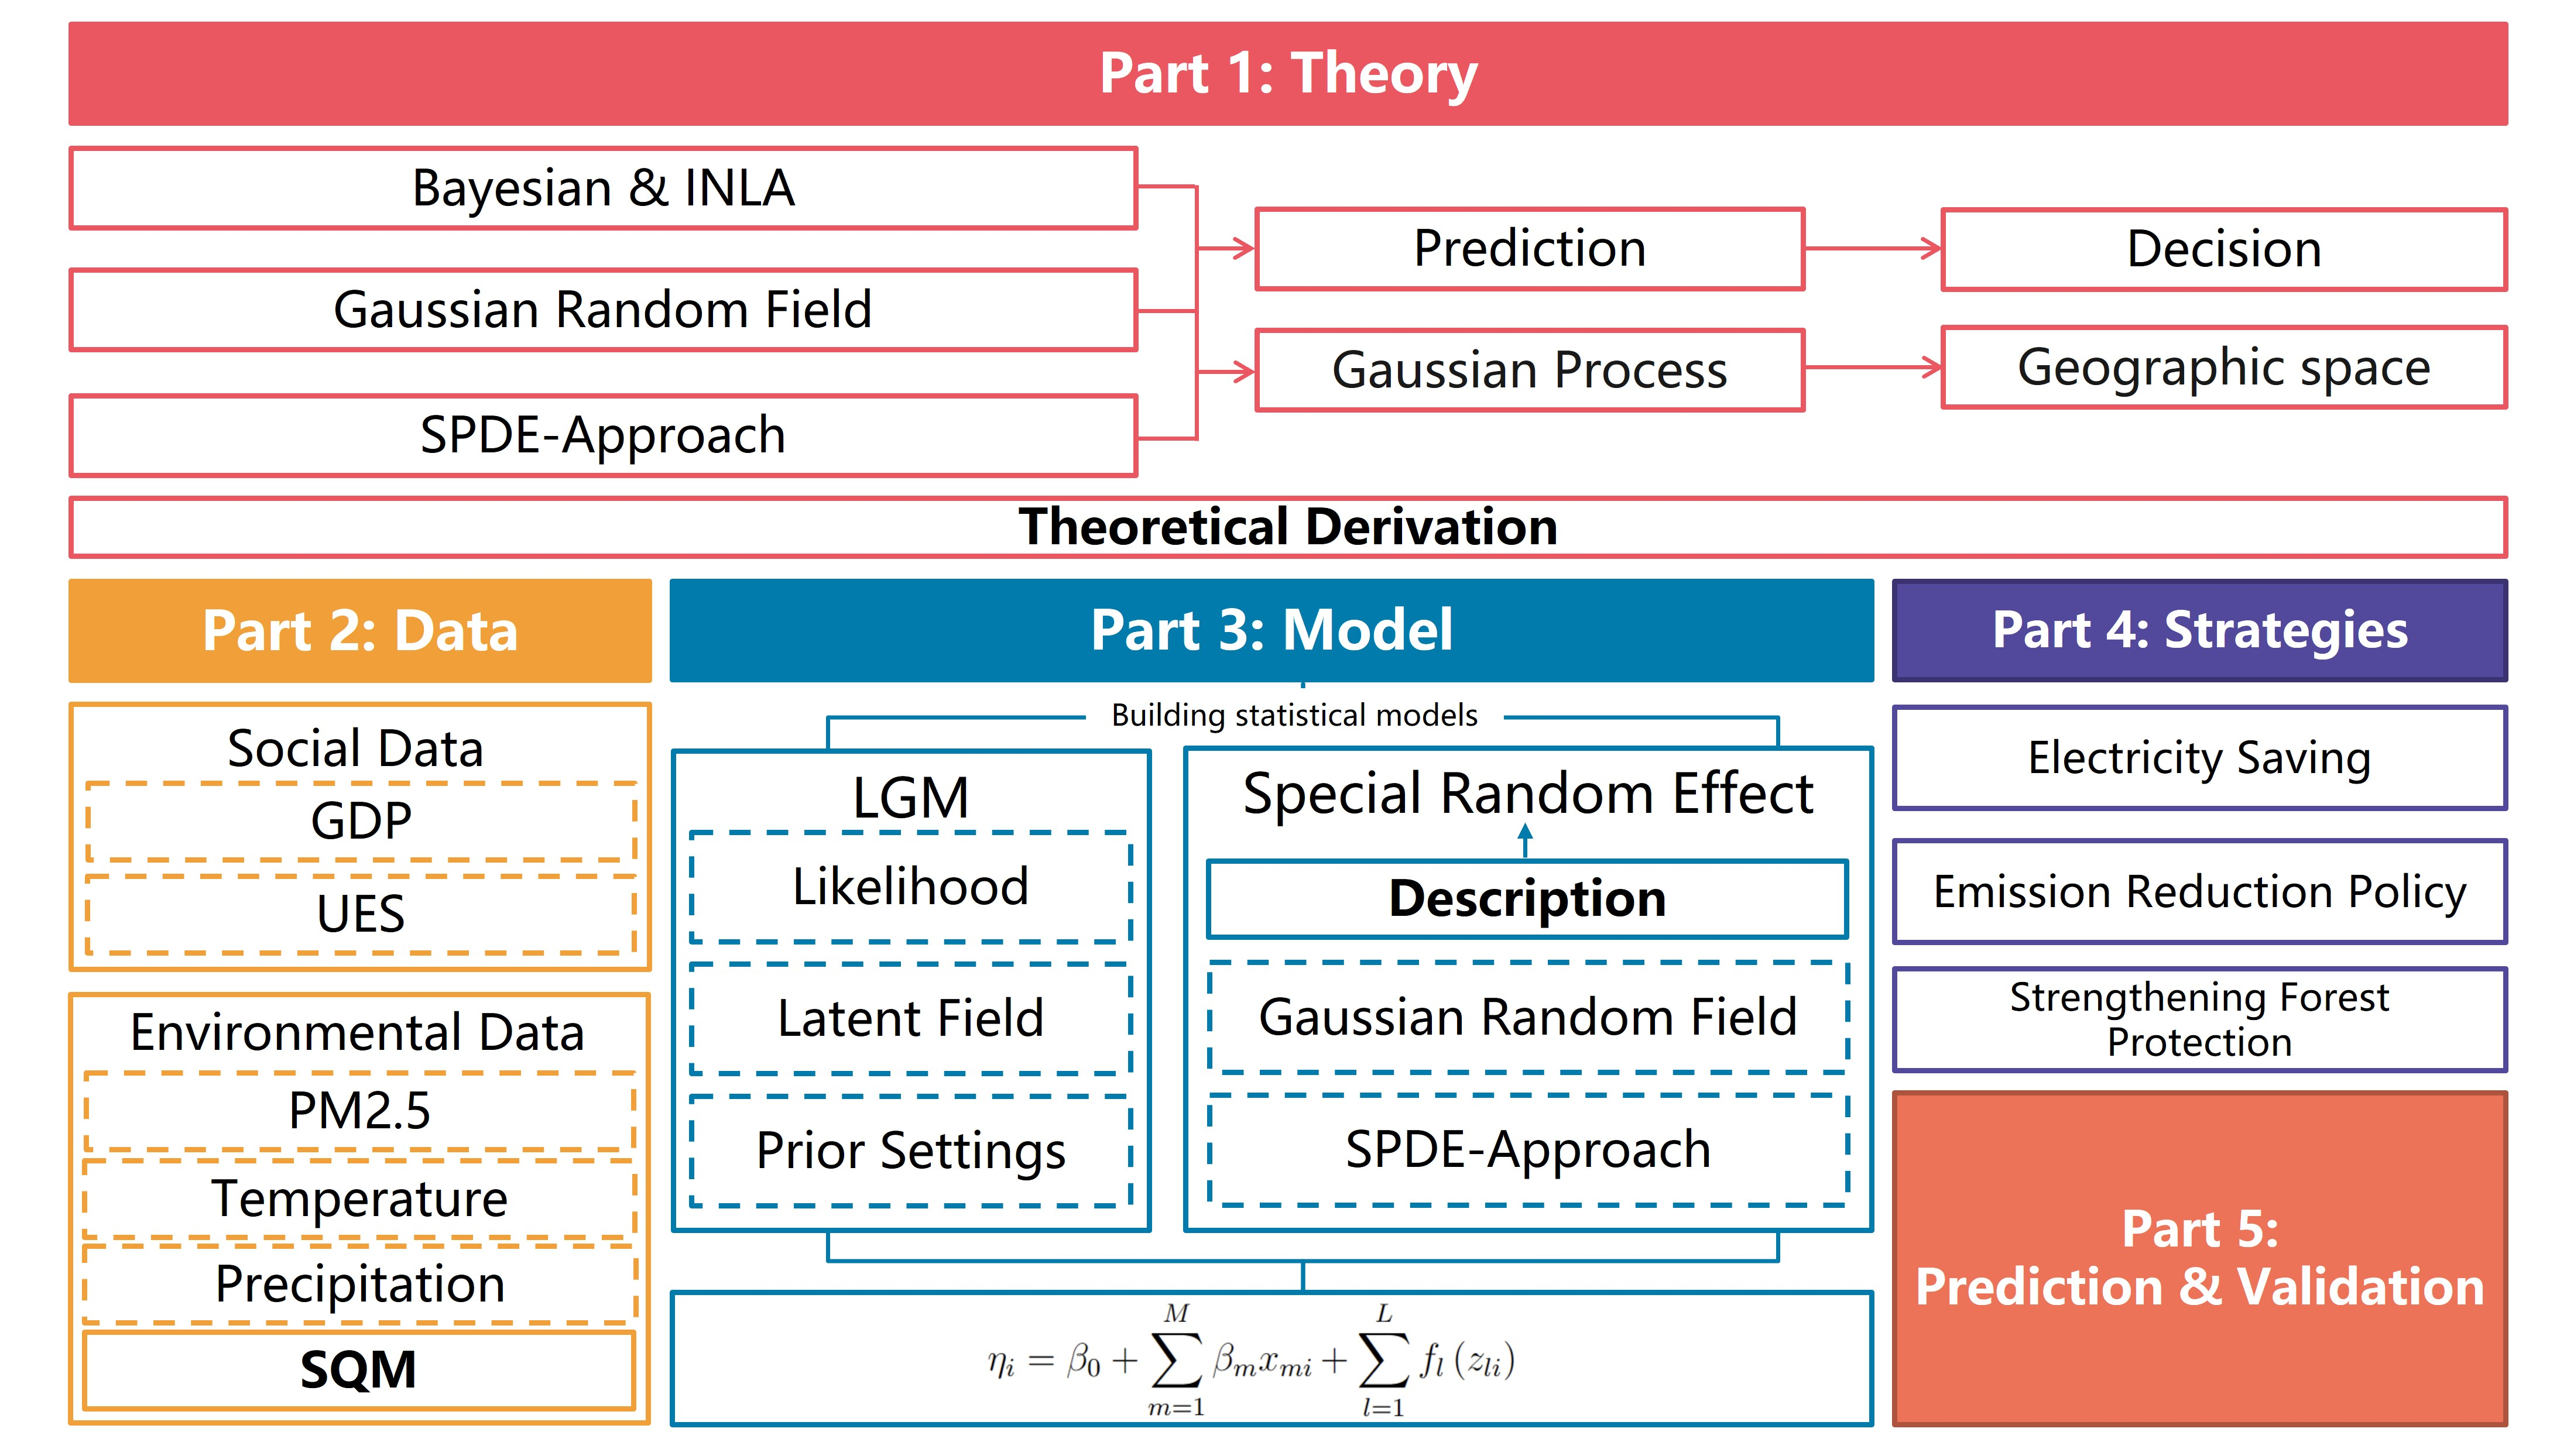
\includegraphics[width=0.8\textwidth]{123.jpg}
    \caption{Overview of the GeoLPBayesian Statistical Computing Framework}
    \label{fig:my_label}
\end{figure}

\section{Preliminary Justification}

\subsection{Assumption}
\subsubsection{Latent Gaussian Models}

\begin{itemize}

    \item Based on requirements and specifications of the problem E. Light pollution will be quantified based on a set of data that needs to contain geometry elements including longitude and latitude. 

    \item The Numerical index for describing the light pollution in our project is the SQM (SKY Quality Meter). The general problem of parametric inference is posited by assuming a probability model for the observed data $\mathbf{y}=(y_1,y_2,...y_n)$. on the location $\mathbf{s}=(s_1,s_2,...s_n)$ in California, as a function of some relevant parameters described by a Gaussian Markov Random Field (GMRF). LGM has three stages which contain the Data model, GMRF prior(latent gaussian field), and hyperprior. For the observed data like SQM which follows a gaussian distribution, we choose the gaussian distribution as our likelihood. 
\end{itemize}

\subsubsection{Additive models} 

\begin{itemize}

\item A very general way to mitigate light pollution is specifying a distribution for observed data SQM $y_{i}$  characterized by a parameter  $\mu_{i}$  (usually the mean) defined as a function of a structured linear predictor  $\eta_{i}$ , presented on a suitable scale, such that  $g\left(\mu_{i}\right)=\eta_{i}$


$$
\eta_{i}=\underbrace{\beta_{0}+\sum_{m=1}^{M} \beta_{m} x_{m i}}_{\text {Fixed effects }}+\underbrace{\sum_{l=1}^{L} f_{l}\left(z_{l i}\right)}_{\text {Random effects }}
$$where $\beta_{0}$  is the overall intercept.\\

\item Generally,$\boldsymbol{\beta}=\left\{\beta_{1}, \ldots, \beta_{M}\right\}$ are used to quantify the effect of the fixed covariates for a broad metric to mitigate light pollution.\\

\item Specifically, in our solution, $$\boldsymbol\beta = \left\{\beta_{PM2.5}, \beta_{SO2},\beta_{CO2},\beta_{Tmean},\beta_{precipitation},
\beta_{population},\beta_{GDP},\beta_{UES}\right\} $$ are specified to evaluate the effect of fixed covariates  $\boldsymbol{x}=\left(\boldsymbol{x}_{1}, \ldots, \boldsymbol{x}_{M}\right)$  on the response.$\boldsymbol{f}=\left\{f_{1}(\cdot), \ldots, f_{L}(\cdot)\right\}$  is a set of functions defined in terms of covariates\\


\item As the data collection suggests, we transform the SQM data to Geostatistical information, so  $f_{i}(\cdot)\sim $ Gaussian field.          Indexes  $\boldsymbol{z}=\left(\boldsymbol{z}_{1}, \ldots, \boldsymbol{z}_{L}\right)$ represent specific Gaussian processes (aka model components) that applied to relax linear relationship of covariates include random effects, temporal and spatial dependence.\\

\end{itemize}


\subsection{Data Description}
Our data is an integrated data set that includes SQM observation$^{[2][9]}$ denoted by variable $yi$ with the covariates $x_{1} ...... .x_{n}$, and after screening the data, we have identified eight sets of covariates relating to environmental and social factors. There is also information on the latitude and longitude corresponding to these points, totaling 3745 SQM observations. Since the covariate data is related to social and environmental factors, it is not possible to achieve a one-to-one correspondence between the covariate observations in the data integration. We have therefore adapted the means of dealing with covariates. We have divided the administrative counties within California so that if multiple locations fall within a county, they will be given the same covariate information to facilitate the integration of the data.

In the calculation of INLA, the dimension of latent effects is best in the range of $10^{2}$-$10^{5}$, which to some extent means our sample size should be less than $10^{5}$. However, if we analyze the global satellite data, the sample size is much higher than $10^{5}$. Therefore, selecting suitable sample information is conducive to our analysis. Here, we picked California. Because it's less than $10^{5}$. Secondly, California is an economically developed region in the United States, with large cities (human factors) and frequent natural disasters (non-human factors), so it is suitable for analysis.

The data we used for our covariates were obtained from authoritative websites: PM$_{2.5}$, SO$_{2}$, and greenhouse gas (CO$_{2}$) data$^{[7][8]}$ were downloaded from the California Air Resources Board. And California county GDP data$^{[6]}$ were obtained from the BEA; regional average temperature and precipitation data are getting from Google Map; population data were cited from Census; and UES data were culled from the California energy commission website. These collected data will be pre-processed and applied to our model.

\begin{figure}[htp]
    \centering
    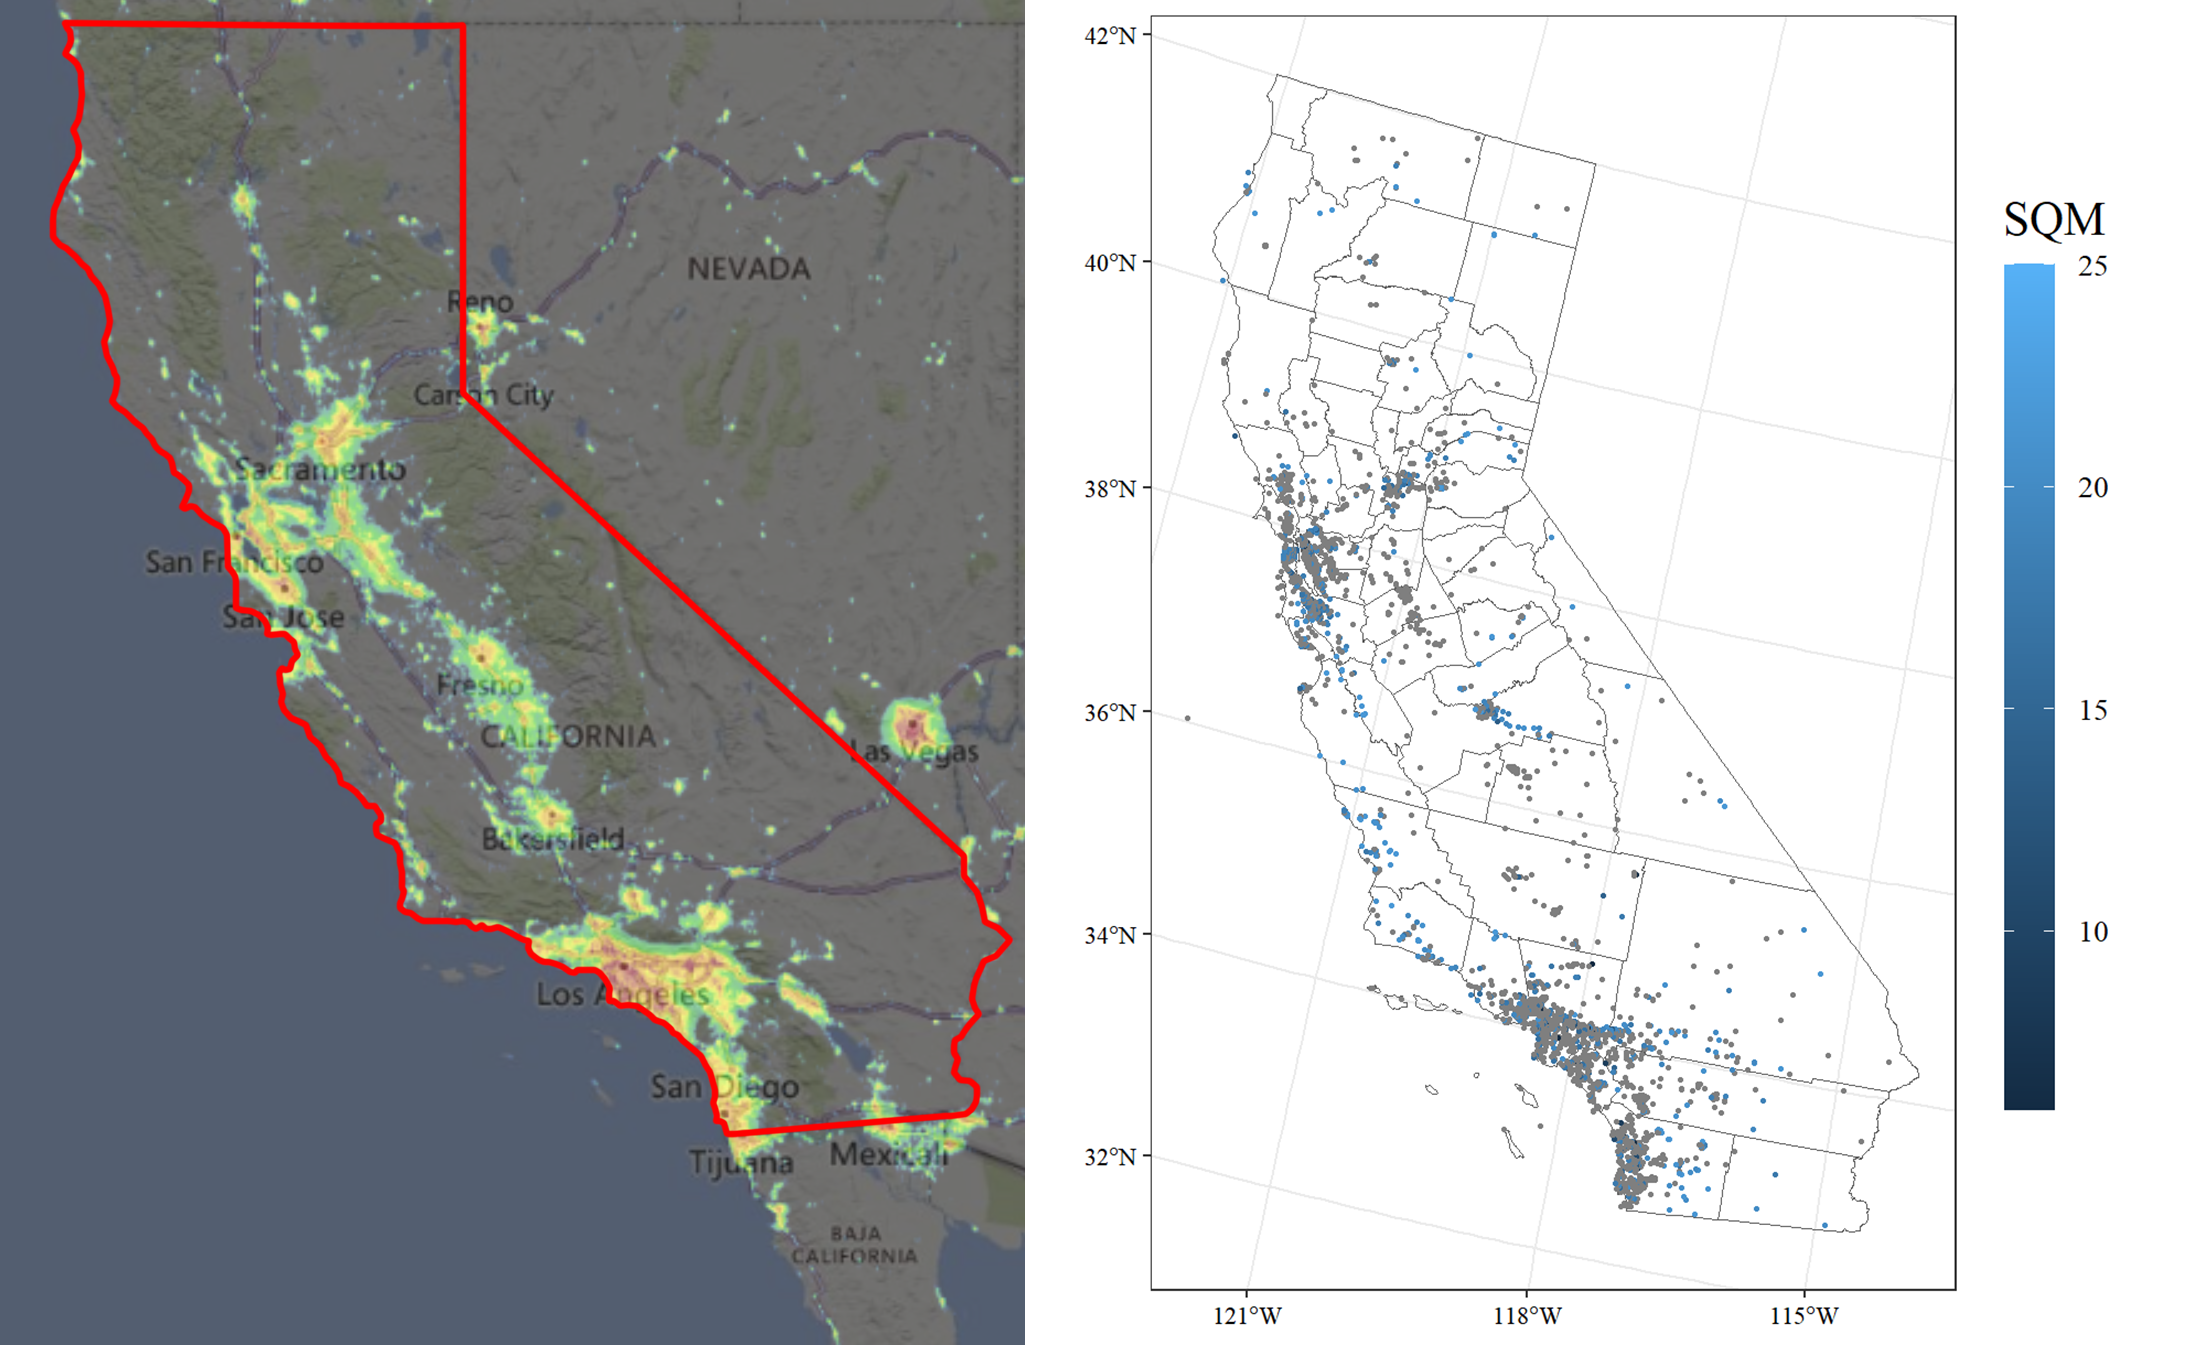
\includegraphics[width=0.7\textwidth]{images/california11.png}
    \caption{The image on the left shows SQM measurements of nighttime lights in California from satellite data $^{[9]}$, while the image on the right shows our collection of SQM data.$^{[2]}$}
    \label{pre1}
\end{figure}


\newpage
\subsection{Notation}

\begin{center}
\begin{tabular}{llll}
\hline
Coefficient & Terminology & Unit & Intervention Strategy \\
\hline
$\beta_{PM2.5}$&Particles in the PM2.5 size &parts per billion (ppb)&     Policy: eg.fuel switching                \\
$\beta_{SO2}$&Sulfur dioxide& $u$g/m^3     & Emission Control                      \\
$\beta_{CO2}$&Carbon dioxide& $u$g/m^3     & Emission Control             \\
$\beta_{Tmean}$&  Average temperature &Fahrenheit degree& Government measurement            \\
$\beta_{precipitation}$& Annual Average Precipitation&mm/h& Government measurement              \\
$\beta_{population}$& Local Population& million &  Policy Management                     \\
$\beta_{GDP}$&Gross domestic product & trillion &  Economic Control                     \\
$\beta_{UES}$& Urban Electricity Supply &kW·h&    Government Policy  \\
\hline 
                                
\end{tabular}

\end{center}


\section{Methodology}

\subsection{Bayesian Inference and INLA}

Let $\mathbf{y}=(y_1,y_2,...y_n)$ be the observed data, then  

Under the Bayesian hierarchical model, the posterior distribution of the unknown parameter $\theta$ derived from the Bayes' Theorem is :
\begin{equation}
\pi(\boldsymbol{\theta} \mid \boldsymbol{y})=\frac{\pi(\boldsymbol{y}, \boldsymbol{\theta})}{\pi(\boldsymbol{y})}=\frac{\pi(\boldsymbol{y} \mid \boldsymbol{\theta}) \pi(\boldsymbol{\theta})}{\int \pi(\boldsymbol{y} \mid \boldsymbol{\theta}) \pi(\boldsymbol{\theta}) d \boldsymbol{\theta}}
\end{equation}
where $\pi(\boldsymbol{y}\mid \boldsymbol{\theta})$ is the likelihood of  $\boldsymbol{y}$. Since $\pi(\boldsymbol{y})$ is the marginal likelihood and free of $\boldsymbol{\theta}$ :
\begin{equation}
    \pi(\boldsymbol{\theta} \mid \boldsymbol{y}) \propto \pi(\boldsymbol{y} \mid \boldsymbol{\theta}) \pi(\boldsymbol{\theta})
\end{equation}
One of the main properties of INLA is that it is used to perform Bayesian inference approximation in latent Gaussian models.  Particularly,  we have three stages for this model construction.
\begin{equation}
\begin{array}{c}
Likelihood:y_{i} \mid \boldsymbol{x}, \boldsymbol{\theta} \sim \pi\left(y_{i} \mid x_{i}, \boldsymbol{\theta}\right), i=1, \ldots, n, \\
Latent Field: \boldsymbol{x} \mid \boldsymbol{\theta} \sim N\left(\boldsymbol{\mu}(\boldsymbol{\theta}), \boldsymbol{Q}(\boldsymbol{\theta})^{-1}\right), \\
Hyperparameters: \boldsymbol{\theta} \sim \pi(\boldsymbol{\theta}),
\end{array}
\end{equation}

with observation $\mathbf(y_1,...,y_n)$, Gaussian latent field $\boldsymbol{x}$ and hyperparameters $\boldsymbol{\theta}$. $\mu(\boldsymbol{\theta})$ is the mean and $Q(\boldsymbol{\theta})^{-1}$ represents the precision matrix of $\boldsymbol{x}$ .  $ y_i$ is connected with effects of various covariates though linear prediction $\eta$ in an addictive way that:
\begin{equation}
\eta_{i} &= \alpha+\sum_{k=1}^{n_{\beta}} \beta_{k} z_{k i}+\sum_{j=1}^{n_{f}} f^{(j)}\left(u_{j i}\right) \\
\end{equation}
\begin{equation}
 \mu_i &= g^{-1}(\eta_i)   
\end{equation}

with $\mu_i$ being the mean of $y_i$. As for $\eta_i$, $\alpha$ is the intercept, {$\beta_k$} is the linear effects of covariates {$z_{ki}$} on $\boldsymbol{y}$.  {$f(.)$} are a set of random effects defined in terms of some covariates {$u_{ji}$}. Here we can see the latent Gaussian variables.

\begin{equation}
    \boldsymbol{x}=\left(\alpha,\left\{\beta_{k}\right\},\left\{f^{(j)}\right\}\right) \mid \boldsymbol{\theta} \sim N(\mu(\boldsymbol\theta), \boldsymbol{Q}(\boldsymbol{\theta})^{-1})))
\end{equation}

corresponding to the second stage of the hierarchical model.  

Based on the approximations above and the Bayesian framework, the typical Integrated Nested Laplace Approximation can be written as:
\begin{equation}
    \tilde{\pi}\left(x_{i} \mid \boldsymbol{y}\right)=\int \tilde{\pi}\left(x_{i} \mid \boldsymbol{\theta}, \boldsymbol{y}\right) \tilde{\pi}(\boldsymbol{\theta} \mid \boldsymbol{y}) d \boldsymbol{\theta}, \\
\end{equation}
\begin{equation}
    \tilde{\pi}\left(\theta_{j} \mid y\right)=\int \tilde{\pi}(\boldsymbol{\theta} \mid \boldsymbol{y}) d \boldsymbol{\theta}_{-j}
\end{equation}

\subsection{The Gaussian random field}

To introduce some notation, let $s$ be any location in a study area $D$ and let $U(\mathbf{s})$ be the random (spatial) effect at that location.  $U(\mathbf{s})$  is a stochastic process, with  $\mathbf{s} \in \mathbf{D}$ , where  $\mathbf{D} \subset \mathbb{R}^{d}$ . Suppose, under this specific framework of project, that  $\mathbf{D}$  is data have been measured at observed locations, over  $d$=2  dimensions within California state.

We denote by  $u\left(\mathbf{s}_{i}\right), i=1,2, \ldots, n.$  a realization of  $U(\mathbf{s})$  at n  locations. Generally, it is assumed that  $u(\mathbf{s})$  has a multivariate Gaussian distribution. If  $U(\mathbf{s})$  is assumed to be continuous over space, then it is a continuously-indexed Gaussian field $(GF)$. To specify the distribution of  $u(\mathbf{s})$ , it is necessary to define its mean and covariance.

To define a correlation function, we specify this on the Euclidean distance between locations. This assumes that given two pairs of points separated by the same distance  $h$ , they will have the same degree of correlation.

Now suppose that  data  $y__{i}$ have been observed at locations  $\mathbf{s}_{i}, i=1, \ldots, n$ . If an underlying $GF$ generated these data, the parameters of this process can be fitted by considering  $y\left(\mathbf{s}_{i}\right)=u\left(\mathbf{s}_{i}\right)$. where data $y_{i}$ are assumed to be realization of  $GF$ with geograhpical data $s_{i}$. In this case, the likelihood function is the multivariate Gaussian distribution with covariance  $\Sigma$.

Moreover, in many conditions, we have measurement errors. $e_{i}$ , i.e., So a more adaptive model is being used.
\begin{equation}
    y\left(\mathbf{s}_{i}\right)=u\left(\mathbf{s}_{i}\right)+e_{i}
\end{equation}

Which $e_{i}$ follows Gaussian distribution with zero mean and variance.



To write the $GF$ (with the Gaussian noise as a nugget effect), $y_{i}$  is assumed to have a Gaussian distribution (with variance  $\sigma_{e}^{2}$  ),$\mathbf{u}$  is modeled as a $GF$. Furthermore, it is possible to consider a multivariate Gaussian distribution for the random effect but it is seldom practical to use the covariance directly for model-based inference.
\begin{equation}
\begin{aligned}
y_{i} \mid \mu_{i}, \sigma_{e} & \sim N\left(y_{i} \mid \mu_{i}, \sigma_{e}^{2}\right) \\
\mu_{i} & =\beta_{0}+u_{i} \\
\mathbf{u} \mid \theta & \sim G F(0, \Sigma)
\end{aligned}
\end{equation}

In the study of Areal data, there are models specified by conditional distributions, implying a joint distribution with a sparse precision matrix. These models are called Gaussian Markov random fields (GMRF).

\subsection{Spatial analysis with the SPDE approach}

In our model, we use the $SPDE$ (Stochastic Partial Differential Equation) approach which could be used to perform the spatial dependence through the $R-INLA$ package to make the prediction of locations where there is a lack of observations. 

As shown in Whittle (1963), a GRF with a $Mat\acute{e}rn$ covariance matrix can be expressed as a solution to the  continuous SPDE:
\begin{equation}
    \left(\kappa^{2}-\Delta\right)^{\alpha / 2}(\tau x(\boldsymbol{s}))=\mathcal{W}(\boldsymbol{s})
\end{equation}

Here,  $x(s)$  is a GRF and $ \mathcal{W}(s)$  is a Gaussian spatial white noise process.  $\alpha$  controls the smoothness of the $GRF$,  $\tau$  controls the variance, and  $\kappa>0$  is a scale parameter.  $\Delta$  is the Laplacian defined as  $\sum_{i=1}^{d} \frac{\partial^{2}}{\partial x_{i}^{2}}$  where  $d$  is the dimension of the spatial domain  $D$. In our case, $d=2$. 

where $\mathbf{s_i}$ and$\mathbf{s_j}$  are two different locations, $ h=||\mathbf{s_i}-\mathbf{s_j}||$ is the Euclidean spatial distance, and $\mathcal{C}(h)$ is the spatial correlation function

\begin{equation}
    \mathcal{C}(h)=\frac{1}{\Gamma(\nu) 2^{v-1}}(\kappa h)^{\nu} K_{\nu}(\kappa h)
\end{equation}

with $K_{v}$ denoting the modified Bessel function of the second kind and order $ \nu>0$ . The parameter $\nu$ measures the degree of spatial smoothness of the process and is often beset with $ \nu =1$ ($\kappa > 0$ is a scaling parameter related to the range $ \rho$, i.e. a distance at which the spatial correlation becomes small. Following Lindgren et al. (2011), we used the empirically derived definition $ \rho = \frac{\sqrt{ 8\nu}}{\kappa}$, with $\rho$ corresponding to the distance where the spatial correlation is close to 0.1, for each $\nu$ . 

In this case, the continuously indexed Gaussian field $x$ can be written as a discretely indexed GMRF (Gaussian Markov random field) with finite basis functions on the mesh:
\begin{equation}
    x(\boldsymbol{s})=\sum_{k=1}^{n} \psi_{k}(\boldsymbol{s}) x_{k}
\end{equation}

In this equation, n is the mesh nodes which means the number of vertices of triangulation. $\psi_{k}(\boldsymbol{.})$ denotes the piecewise linear basis functions. ${x_k}$ are zero-mean Gaussian distributed weights and the joint distribution $\mathbf{x} = (x_1,...,x_n) \sim N(0,Q^{-1}(\tau, \kappa))$ which could make the approximation of the solution $x(\mathbf{s})$ of the $SPDE$ from the mesh nodes to the other spatial locations. 

\begin{figure}[htp]
    \centering
    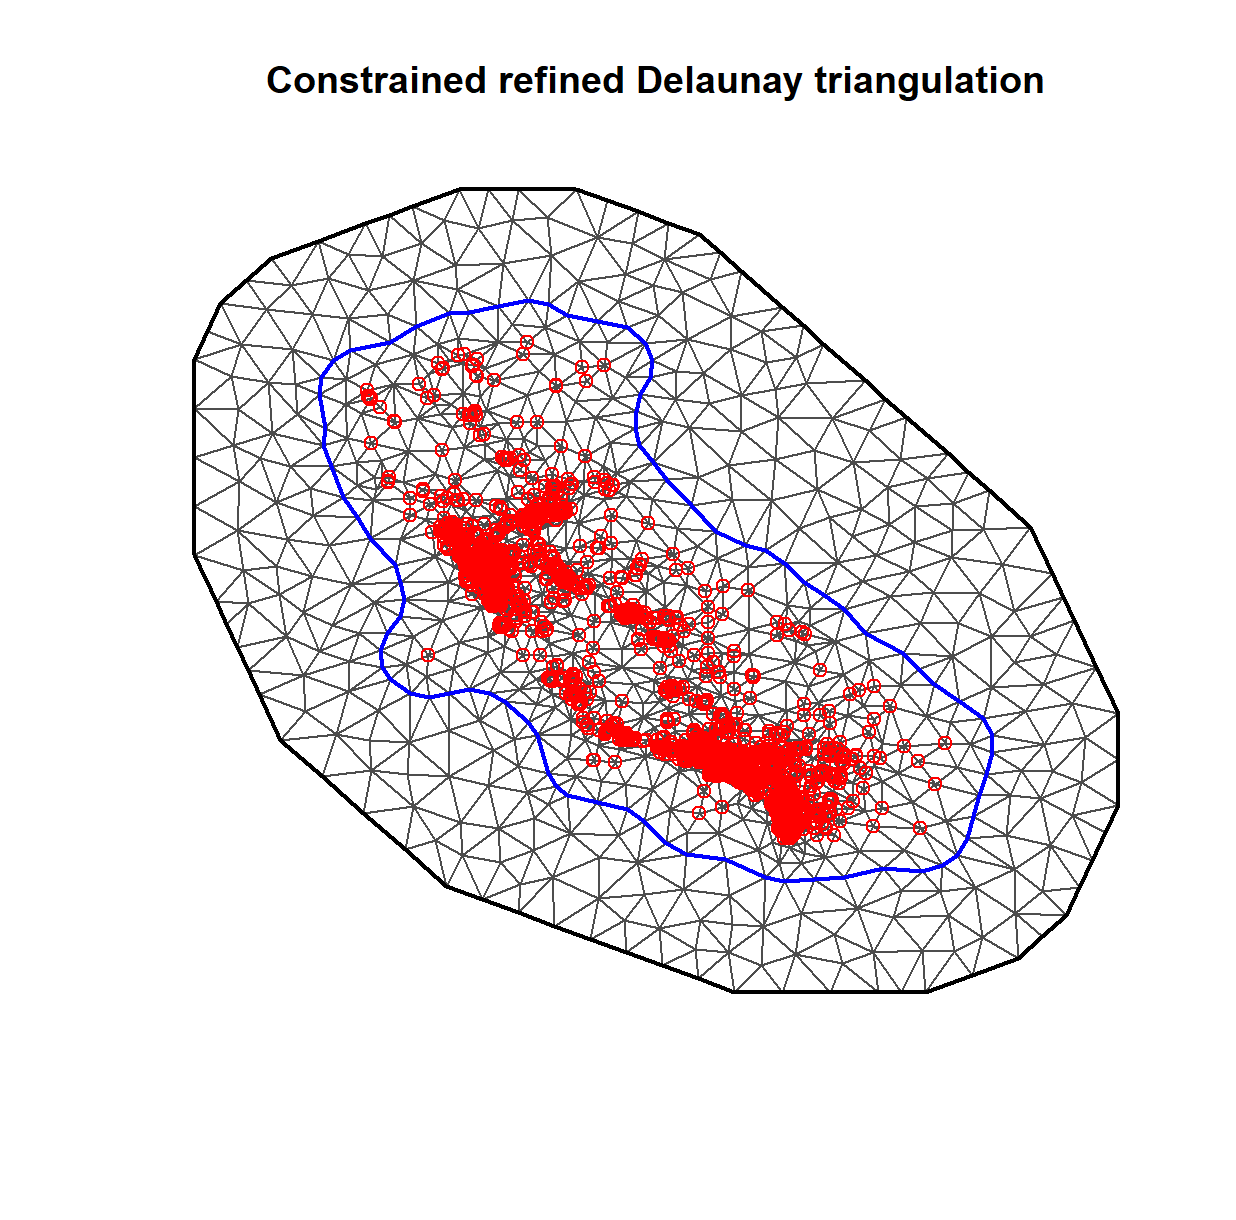
\includegraphics[width=0.5\textwidth]{images/mesh0.png}
    \caption{The mesh used to build for California with SPDE approach}
    \label{pre1}
\end{figure}


\section{Bayesian Hierarchical Model Building}

\subsection{likelihood}


During this section, we will talk about our statistical model in a more specific way.  Let $y(\boldsymbol{s})$ be our response value. Namely, the SQM value has been observed. Let $\boldsymbol{s}_{i}$ be the spatial location and $\boldsymbol{s} \in \mathcal{S}$ which is California, containing 3725 locations$^{[12]}$.

The Bayesian Hierarchical model is constructed into three parts, They are \textbf{likelihood}, \textbf{latent field}, \textbf{prior}. Here will analyze these three parts.$^{[13]}$

With the data characteristics, we choose the gaussian distribution as our likelihood function. \\Within the skewness calculation. We find that the skewness of the SQM data is near 0.07 which is close to 0.

The Gaussian distribution is
\begin{equation}
    f(y)=\frac{\sqrt{s \tau}}{\sqrt{2 \pi}} \exp \left(-\frac{1}{2} s \tau(y-\mu)^{2}\right)
\end{equation}

for continuously responses  y  where $\mu$  : is the the mean.  $\tau$  : is the precision.  $s$:  is a fixed scaling,  $s>0$. Their corresponding domains are $ -\infty<\mu<\infty, \s>0, \tau>0$.  The mean is linked to the linear predictor by $\eta$. 



Linear predictor $\eta$ connects the response variable which is the observed data and several effects of the model by the link function which is the identity function in our case (i.e., $\eta=\mu(\boldsymbol{s})=E(y(\boldsymbol{s}$). 

Since we have fixed effects from many aspects. From the Enviroment : We have PM2.5, SO2, CO2, Temperature mean, and precipitation. From the  social aspect, we have the population, GDP, and Urban electricity supply for each California county. Then we add the spatial random effect which uses the SPDE approach. Also, the error items for our linear predict model should be considered. 

\textbf{Model:}

\begin{equation}    
\eta_{1}(s) &=\boldsymbol{z}(s){\boldsymbol\beta^{T}}+ u_{SPDE}(s)+\varepsilon(\boldsymbol{s})\\
\end{equation}
\begin{equation}
u(s)  &\sim \mathcal{G} \mathcal{P}_{2 \mathrm{D}-\operatorname{SPDE}}.
\end{equation}


In our model. The $\boldsymbol\beta = \left\{\beta_{PM2.5}, \beta_{SO2},\beta_{CO2},\beta_{Tmean} ,\beta_{precipitation},\beta_{population},\beta_{GDP},\beta_{UES}\right\} $ 

\subsection{Gaussian Latent Field}

The second part of the model consists of the Gaussian latent field. Let $\boldsymbol{x}$ be latent effects, which is also the Gaussian latent field, and we assume that it follows:
\begin{align}
     \boldsymbol{x} \mid \boldsymbol{\theta} \sim N\left(\boldsymbol{0}, \boldsymbol{Q}(\boldsymbol{\theta})^{-1}\right),
\end{align}
where the $\boldsymbol{Q}(\boldsymbol{\theta})^{-1}$ is the precision matrix of $\boldsymbol{x}$ and $\boldsymbol{\theta}$ is the hyperparameter in the model. $^{[14]}$

\subsection{Prior Definition}
A key point in Bayesian Inference is that the prior distribution is required during the calculation of posterior density with the sample $\left\{y_{1},..y_{n}\right\}$. We need to decide the prior distribution for the precision parameter $\tau$ in Gaussian distribution, the coefficients for fixed effects $\boldsymbol{\beta}$, and parameters $\nu_{SPDE}$, $\rho_{SPDE}$, $\sigma_{SPDE}$, $\tau_{SPDE}$ in the SPDE approach. $\nu_{SPDE}$ controls the smoothness, $\tau_{SPDE}$ controls the variance, and the INLA has the default priors and also allows users to make their own decisions based on the empirical decision.\\

We use the vague gaussian distribution to define our $\boldsymbol{\beta}$ prior. log-gamma distribution for $\tau_{gaussian}$ and $\tau_{SPDE}$. The Penalized Complexity (PC) priors are for the $\rho_{SPDE}$ and $\sigma_{SPDE}$.



\subsubsection{Gaussian prior}
The normal Gaussian distribution has a density
\begin{equation}
    \pi(\theta) = \left(\frac{\tau}{2 \pi}\right)^{1 / 2} \exp \left(-\frac{\tau}{2}(\theta-\mu)^{2}\right)
\end{equation}

\\
  for continuous $\theta$ where $\mu$ :is the mean $\tau$ :is precision.

\subsubsection{log-gamma prior}
The Gamma distribution has a density
\begin{equation}
    \pi(\tau)=\frac{b^{a}}{\Gamma(a)} \tau^{a-1} \exp (-b \tau)
\end{equation}

for  $\tau>0$  where:
 $a>0$  is the shape parameter, and
 $b>0$  is the inverse-scale parameter.
The mean of  $\tau$  is  $a / b$  and the variance is  $a / b^{2}$ , and we denote this distribution  $\operatorname{Gamma}(a, b)$ . The variable  $\theta$  has a  $\log \operatorname{Gamma}(a, b)$  distribution, if  $\theta=\log (\tau)$  and  $\tau$  is  $\operatorname{Gamma}(a, b)$  distributed.

As we talk about the fixed effects like the covariates for two main aspects, the Environment and the Social aspects. And we also consider the random effects as the spatial analysis with the SPDE approach. Here we give the Bayesian Hierarchical Model. 

\begin{center}
\begin{align}
     y (s_{i})&\sim N (\mu(s_{i}),\tau)\\
     E(y\left(\boldsymbol{s}_{i}\right))&=\eta\left(\boldsymbol{s}_{i}\right)\\
\eta\left(\boldsymbol{s}_{i}\right)&=\boldsymbol{z}\left(\boldsymbol{s}_{i}\right)\boldsymbol{\beta^T}
+\boldsymbol{g}_{SPDE}\left(\boldsymbol{s}_{i}\right)+\varepsilon\left(\boldsymbol{s}_{i}\right)
\\
 \boldsymbol{x} \mid \boldsymbol{\theta} &\sim N\left(\boldsymbol{0}, \boldsymbol{Q}(\boldsymbol{\theta})^{-1}\right)
 \\
 \boldsymbol{\theta} &\sim \pi(\boldsymbol{\theta}).
\end{align}
\end{center}





\section{Results and Decision Making}
\subsection{Baseline model performance without intervention strategy}
\subsubsection{Statistical Analysis for posterior distribution under fixed effect} 


\begin{center}
\begin{tabular}{llllll}
\hline
Coefficient & mean & SD & 0.025quant & 0.5quant & 0.975quant\\
\hline
$\beta_{UES}$& 8.330 & 0.050 & 8.122 & 8.338 & 8.493         \\
$\beta_{PM2.5}$& 3.438 & 0.318 & 2.873 & 3.416 & 4.124      \\
$\beta_{SO2}$& 2.566& 0.580 & 1.670 & 2.575 & 3.767            \\
$\beta_{CO2}$& 2.464 & 1.232 & 1.986 & 2.471 & 2.872            \\
$\beta_{precipitation}$& 2.408 & 0.445 & 1.693 & 2.611 & 3.507          \\
$\beta_{Tmean}$& 1.474 & 0.231 & 0.995 & 1.571 & 1.875              \\
$\beta_{population}$& 0.081 & 0.058 &  0.055 & 0.081 & 0.143                \\
$\beta_{GDP}$& 0.027 & 0.014 & -0.005 & 0.025 & 0.042                    \\
\hline 
                                
\end{tabular}
\end{center}

In the Latent Gaussian model, the $\boldsymbol{\beta}$ will have vague Gaussian priors. The posterior distribution of $\boldsymbol{\beta}$ will be computed and shown in the above table. Here we use the posterior mean as our estimated value for the coefficient. For each observed $y_{i}$, it will have a specific distribution characterized by a parameter  $\mu_{i}$  (usually the mean) defined as a function of a structured linear predictor  $\eta_{i}$. In the additive model, when the coefficients get larger, it will have a more significant impact on the linear predictor.

\begin{figure}[htp]
    \centering
    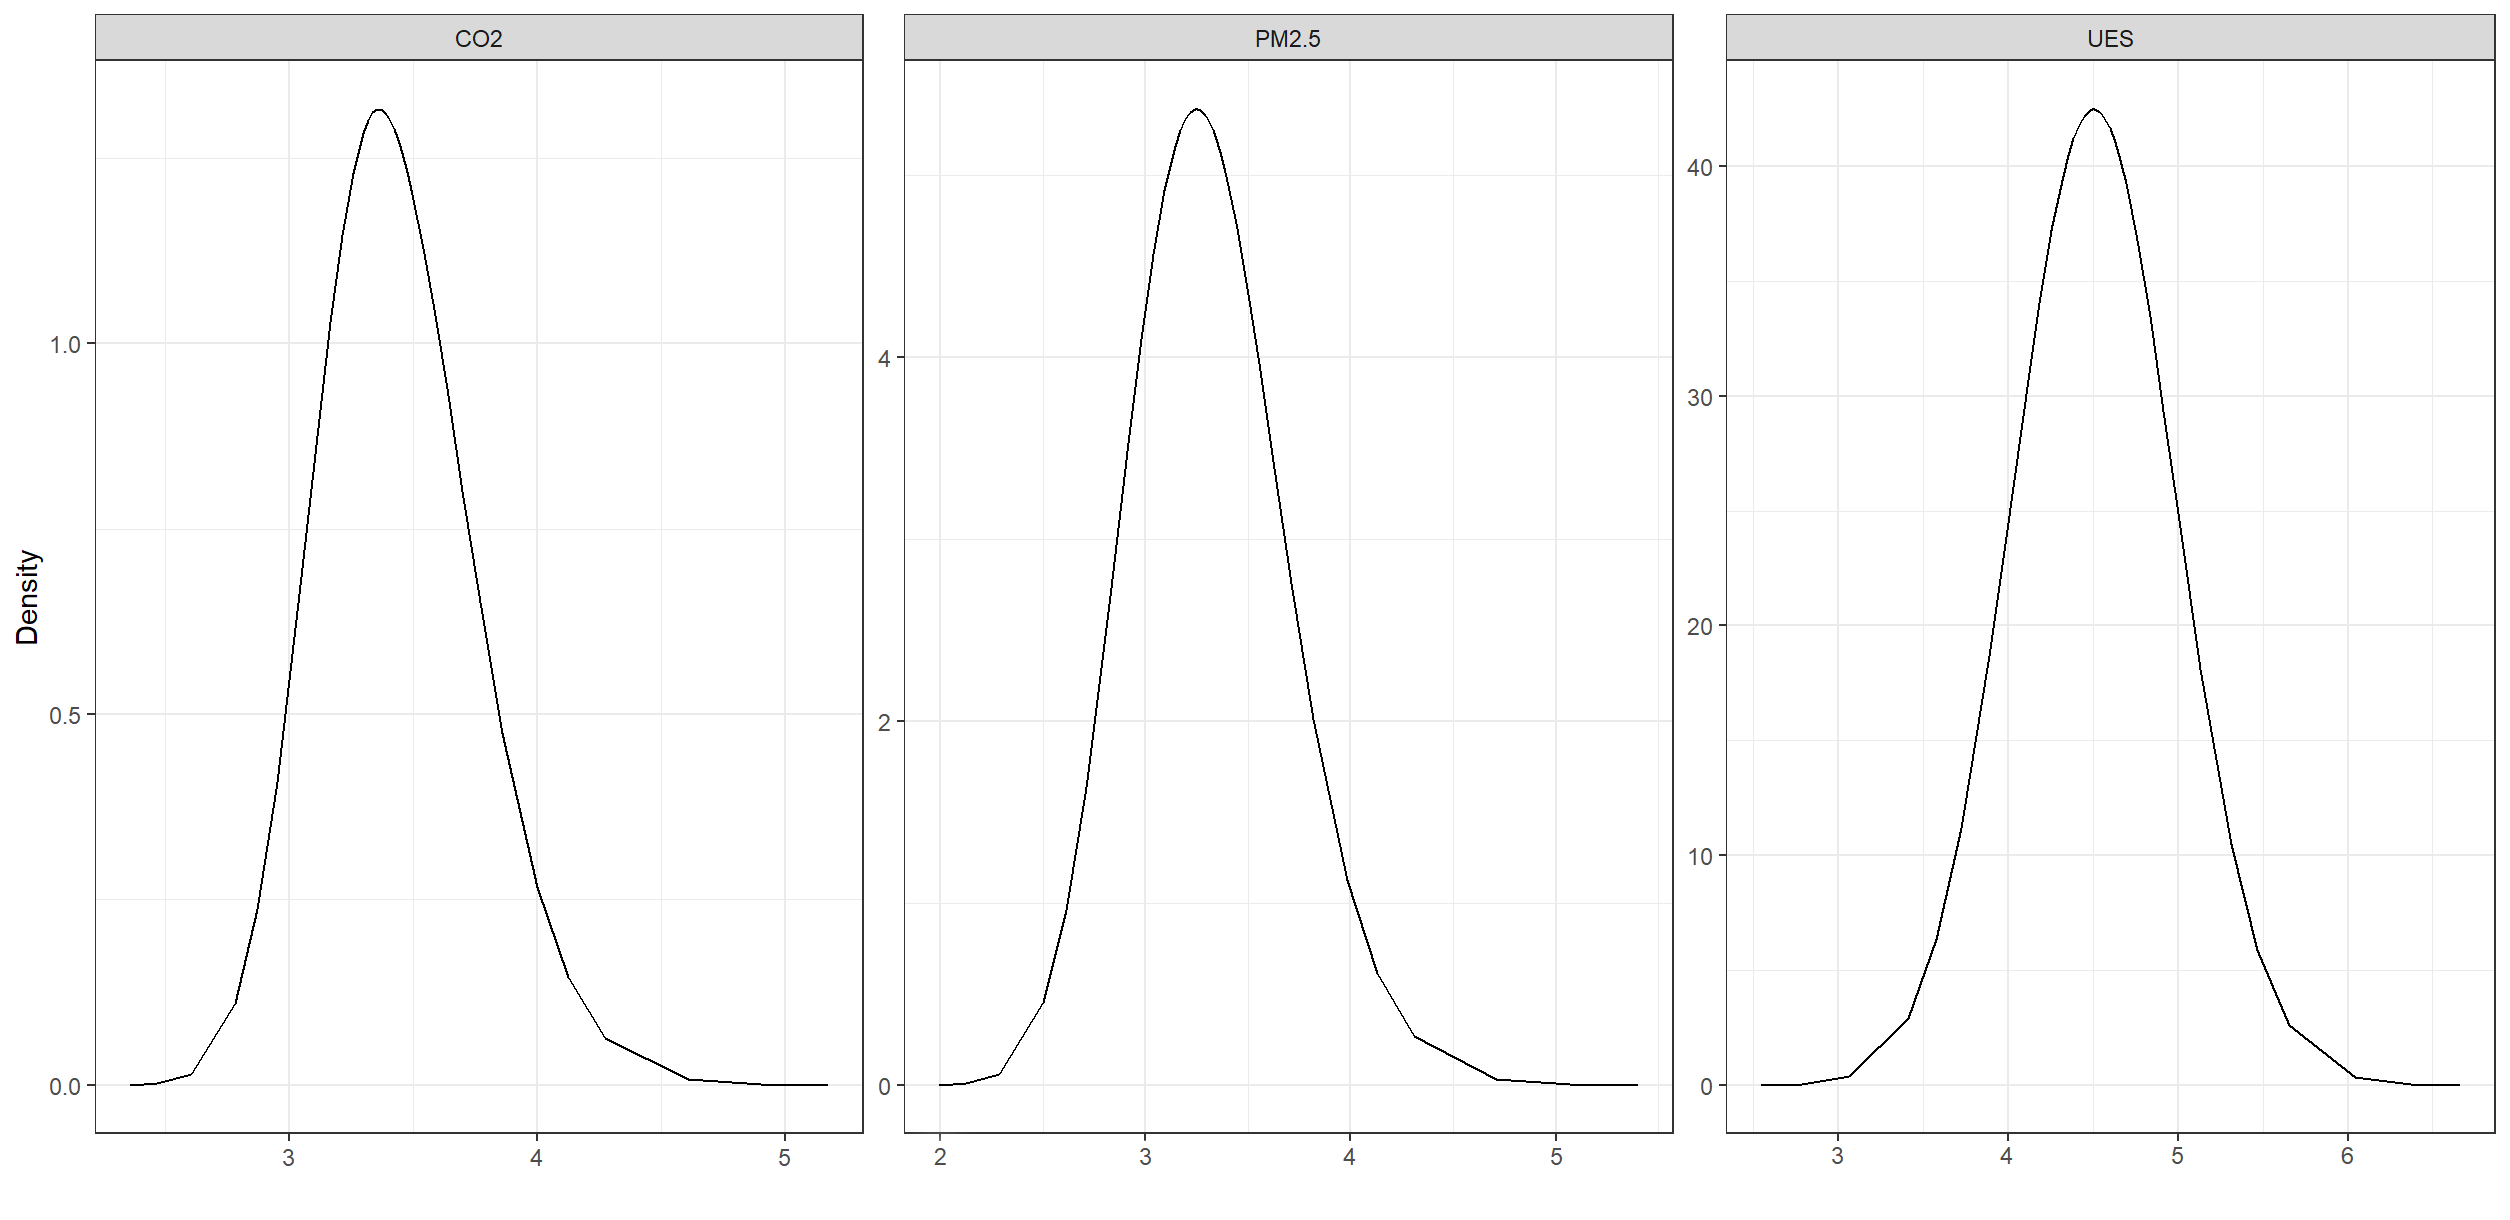
\includegraphics[width=0.5\textwidth]{images/posterior.png}
    \caption{posterior distribution for the three coefficients}
    \label{pre1}
\end{figure}

\subsection{Strategy Development}
To be more specific, UES(Urban Electricity Supply) is controlled by state governments and the awareness of citizens; PM2.5 and SO2 are indicators of air quality with each reflecting the progression and severity of light pollution. They intervened through both intellectual and individual endeavors, such as implementing strategies to limit electricity use, utilizing governmental legislation to control emissions, promoting novel fuel material, etc.


\subsubsection{Spatial prediction and Excursions function for light pollution level}

In the model computation, we demonstrate 11161 points and initially filled them with NA values, which contain cover the whole area of California. In the Bayesian hierarchical model, we shall compute the marginal distribution of latent effect $\boldsymbol{x}$ to get the predicted value for each NA. 

\begin{figure}[htb]
    \centering
    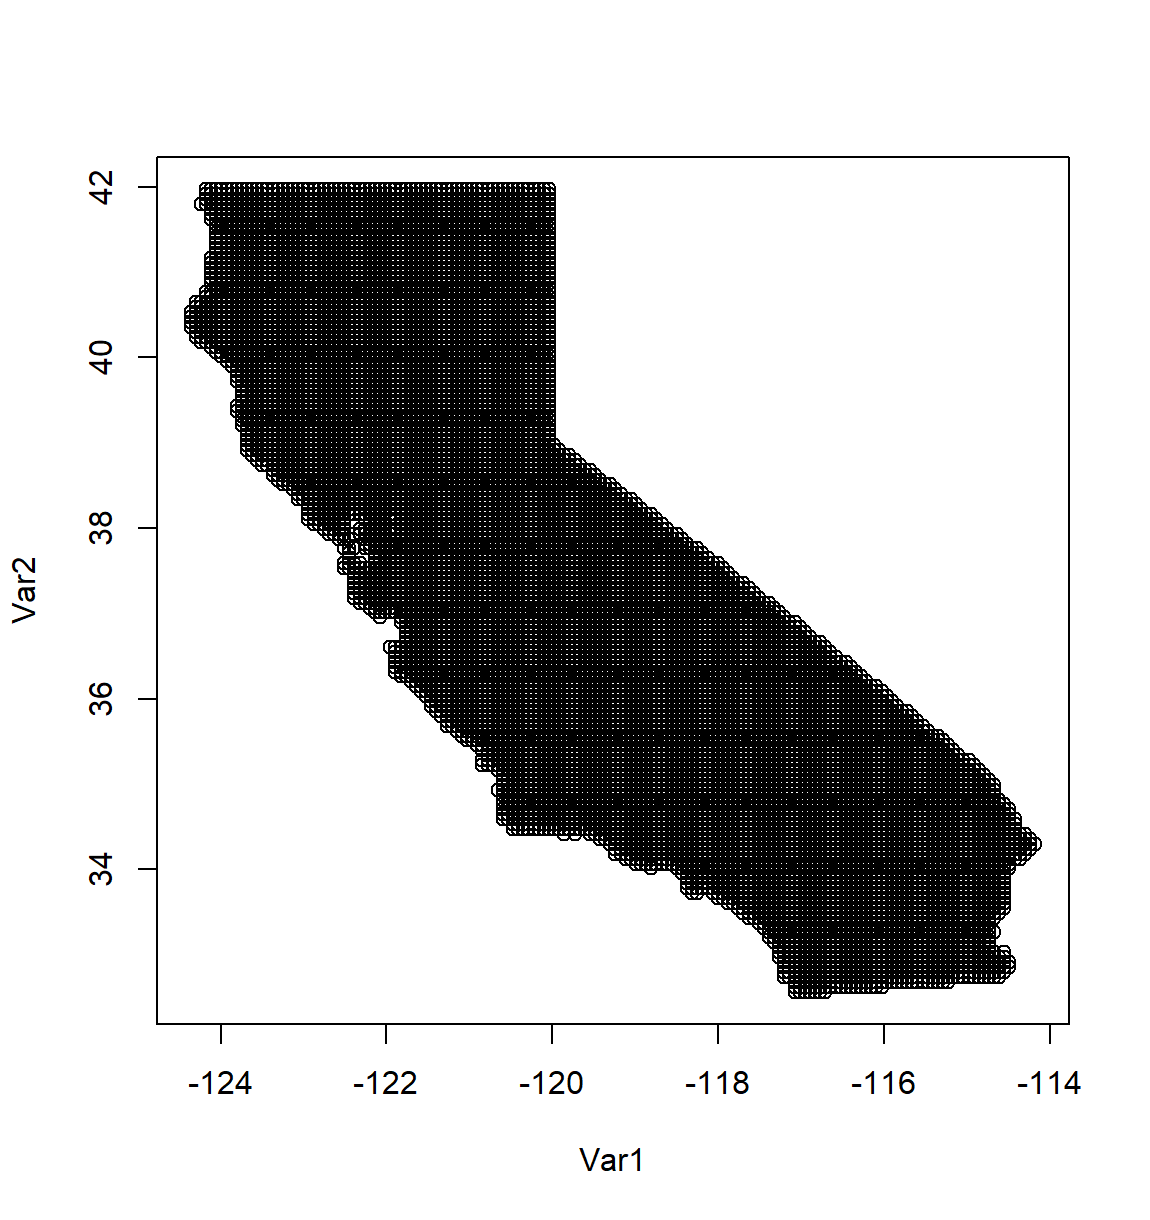
\includegraphics[width=0.35\textwidth]{images/11361.png}
    \caption{11161 NA points cover the whole of California}
    \label{pre1}
\end{figure}
\newpage
Excursion functions region identifications and predictive concentration level plots are important tools in light pollution studies. Bolin and Lindgren (2015) proposed the positive  $\left(\mathrm{E}_{u, \alpha}^{+}(X)\right)$ that determines the largest set that simultaneously exceeds or below the risk level  (u)  with a small error probability  $(\alpha)$ , employing a parametric family and sequential importance sampling method for estimating joint probabilities. To visualize the excursion sets simultaneously, we apply the positive excursion functions in our situation,  $F_{u}^{+}(s)=1-\inf \left\{\alpha \mid s \in \mathrm{E}_{u, \alpha}^{+}\right\}$.
\textbf{The positive excursion function often shows increased odds for the site ($s_{0}$) to concurrently surpass the danger threshold ($u$),which is indicated in our project to determine the likelihoods for the California sites that are more likely to have light pollution than the acceptable level.}

\begin{figure}[H]
\centering
\subfigure[]{
\begin{minipage}[t]{0.5\linewidth}
\centering
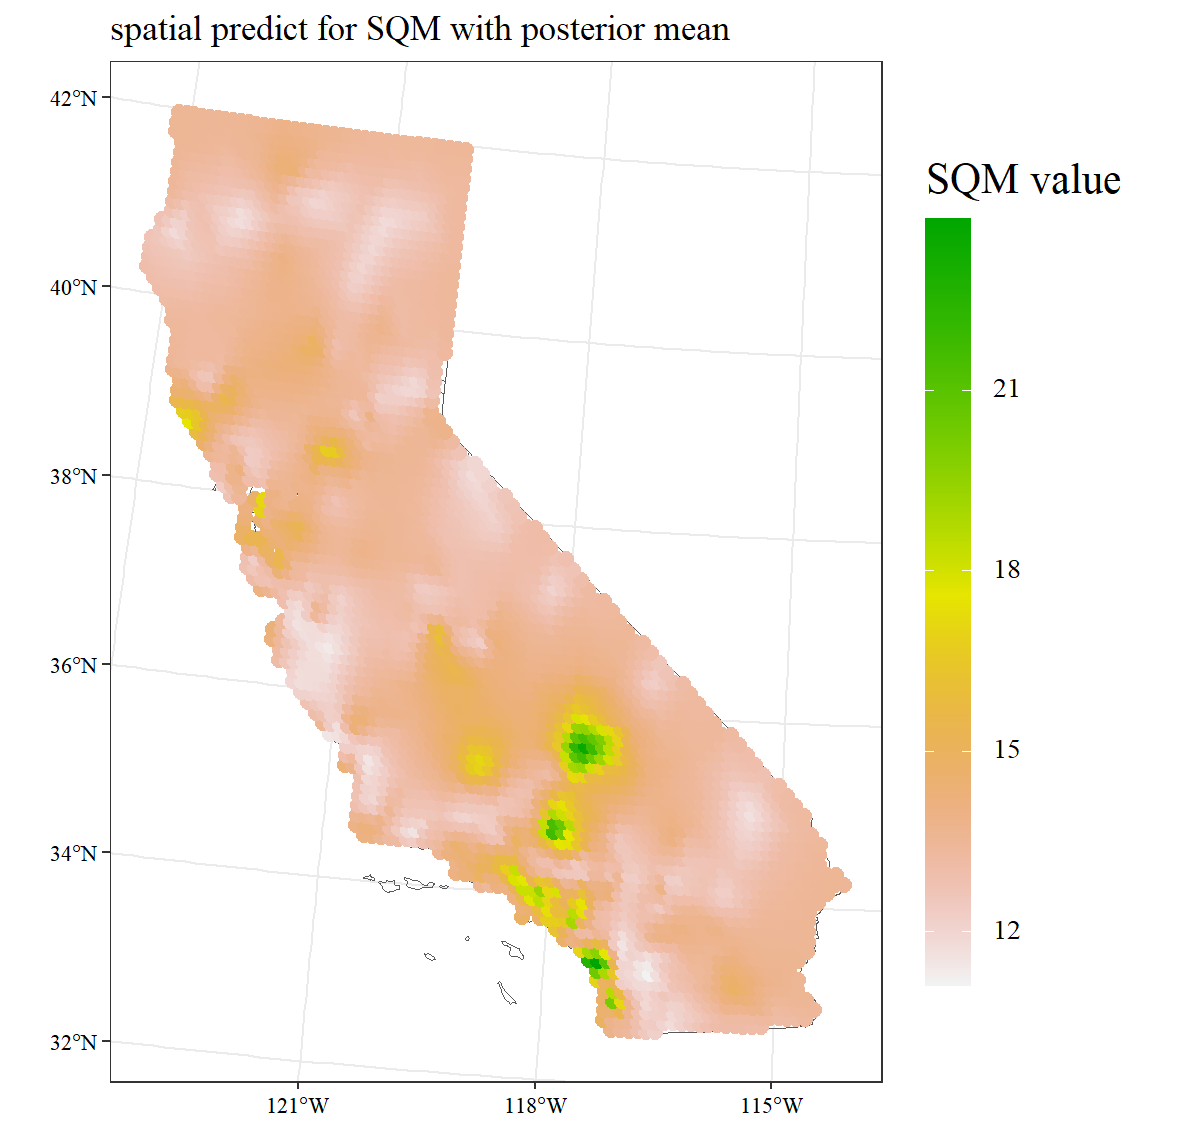
\includegraphics[width=0.9\linewidth]{images/toy.png}
%\caption{fig2}
\end{minipage}%
}%
\subfigure[]{
\begin{minipage}[t]{0.5\linewidth}
\centering
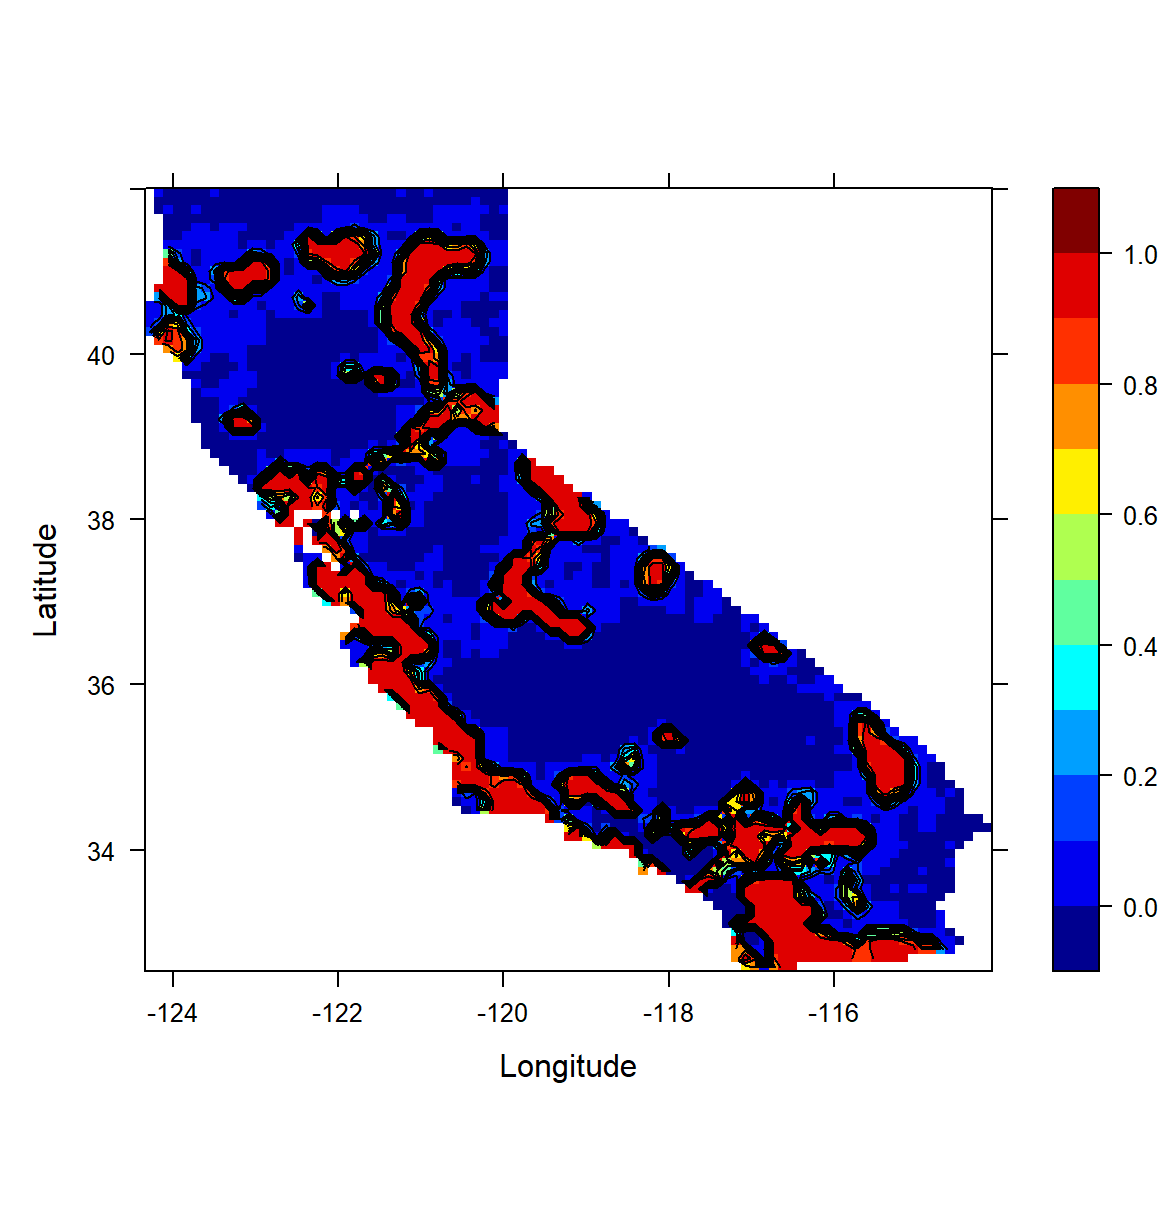
\includegraphics[width=0.9\linewidth]{images/excursions.png}
%\caption{fig2}
\end{minipage}
}%
\centering
\caption{ Left: 11161 points with our spatial prediction; Right: Positive Excursion function}
\end{figure}

\subsection{Analysis of impacts after intervention}
\subsubsection{Case study for two selected locations}

\begin{itemize}

\item Here, we define the study using four distinct regions (protected, rural, suburban, urban)in \textbf{southern California} under the prediction and representation of our model. We estimate the precision of our model over regions based on the standard deviation of the \textbf{spatial random effect}.

\item Out of the four different regions, based on our validation and training sets, we picked two regions(rural, urban) with higher prediction precision for subsequent analysis and strategy comparison.

\item For rural and urban locations, respectively, we shall decide in these two areas in the context of the vectorization of discreet location, with the techniques of decision-making for intervention strategy including policy adjustment, public education, etc. The examination of these policies in our model should \textbf{lead to a shift in the covariate data}, which will additionally impact both our model and the data in terms of intervention strategies.

\item Our objective is to determine the \textbf{significance of the change in the covariate data} before analyzing which of our choices had the \textbf{most significant impact on the regional SQM change}.

\begin{figure}[htb]
    \centering
    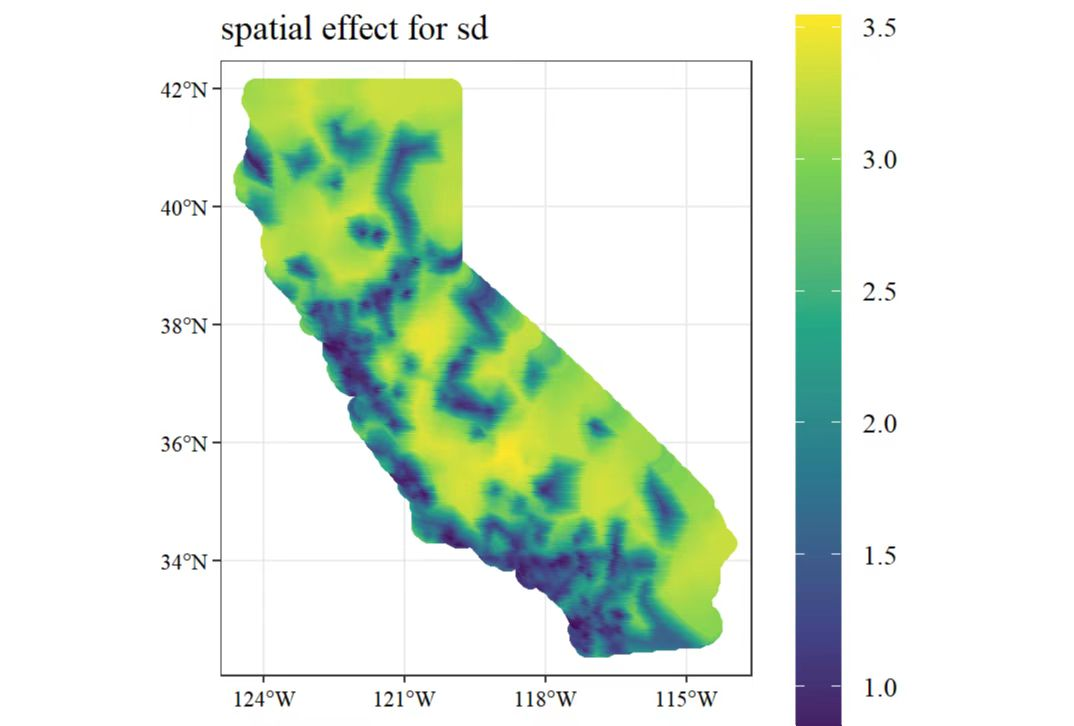
\includegraphics[width=0.5\textwidth]{images/random effect sd.jpg}
    \caption{Spatial random effect stand deviation}
    \label{pre1}
\end{figure}

\begin{figure}[htb]
    \centering
    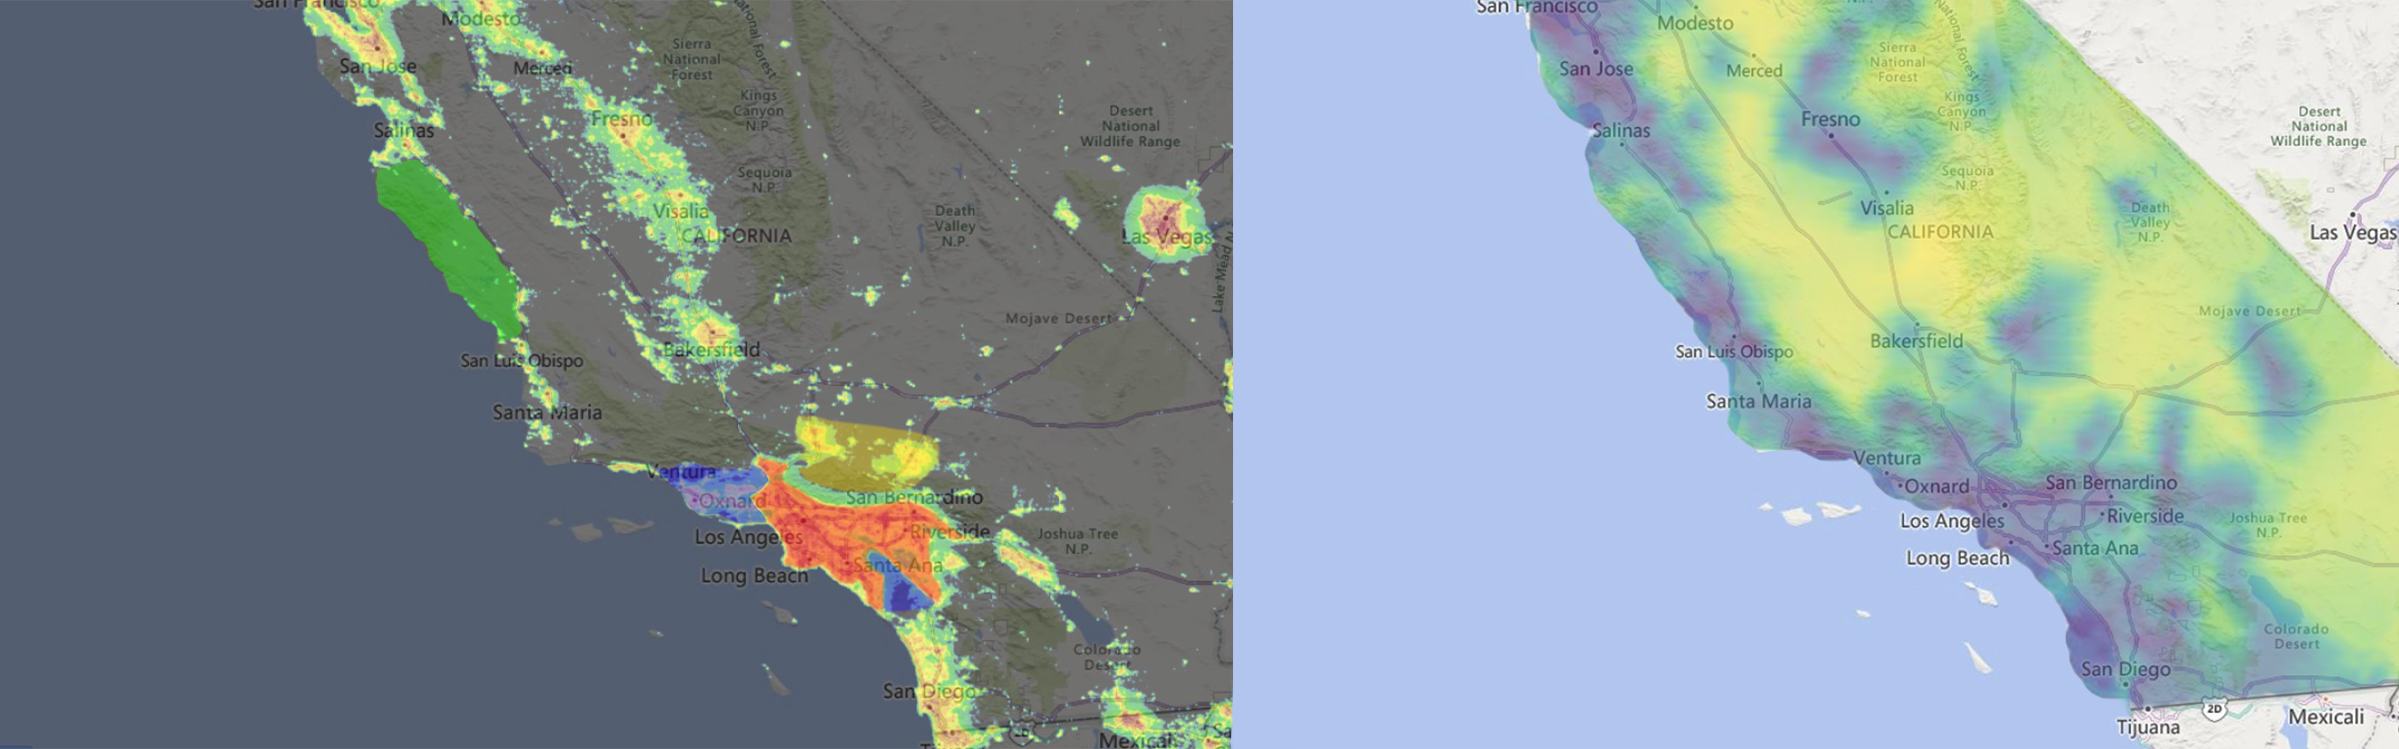
\includegraphics[width=0.9\textwidth]{images/compare.png}
    \caption{The left figure shows the 4 different locations: green represents protected land location, blue represents suburban community, red represents urban community, yellow represents rural community, the right figure shows us the model spatial random effects stand deviation }
    \label{pre1}
\end{figure}

\end{itemize}

\subsubsection{Determine the most significant strategy for Rural community}
\begin{center}
\begin{tabular}{llllll}
\hline
Coefficient & mean & SD & 0.025quant & 0.5quant & 0.975quant\\
\hline
$\beta_{UES}$& 3.128 & 0.789 & 1.581 & 3.128 & 4.674         \\
$\beta_{PM2.5}$& 1.094 & 0.030 & 1.007 & 1.040 & 1.102      \\
$\beta_{SO2}$& 0.348 & 0.022 & 0.305 & 0.348 & 0.391            \\
\hline 
                                
\end{tabular}
\end{center}

\begin{figure}[htp]
    \centering
    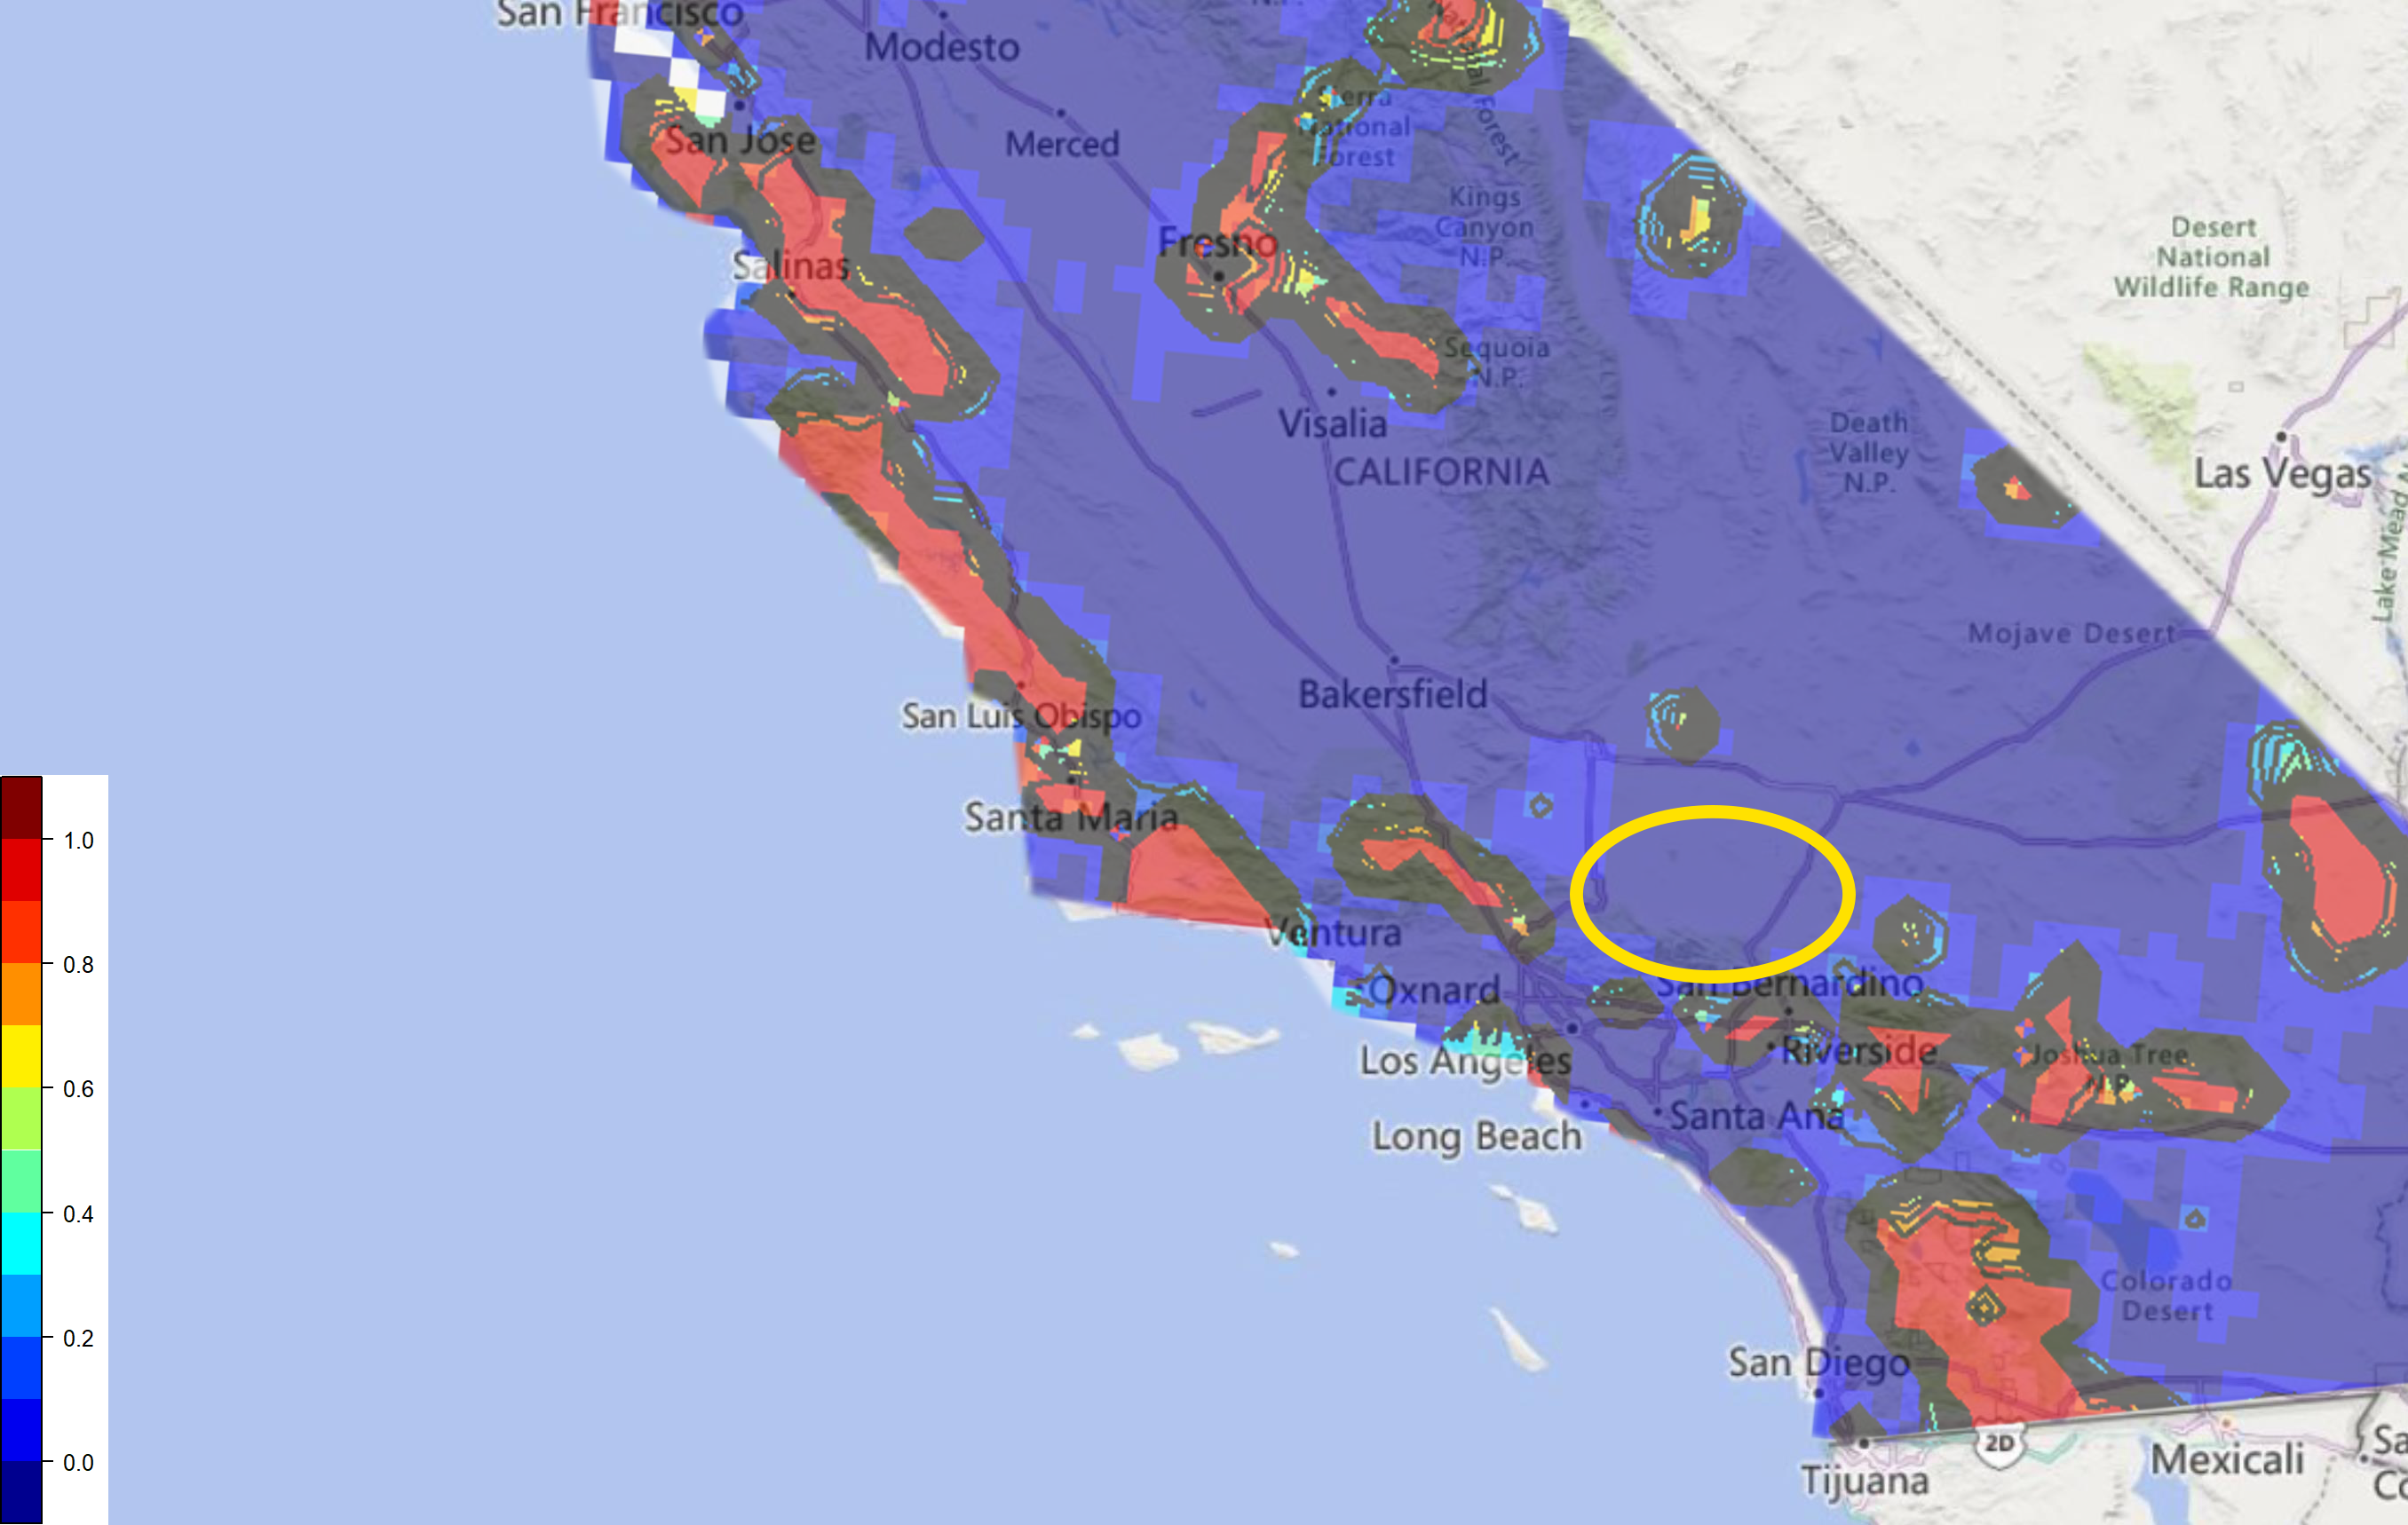
\includegraphics[width=0.5\textwidth]{images/qwq.png}
    \caption{Excursion function for Rural community}
    \label{pre1}
\end{figure}
\newpage
After the computational simulation of three selected strategies for the rural location, the countryside around Lancaster was chosen as our target to quantify the effects of UES, PM2.5$^{[7]}$, and SO2 $^{[8]}$ with changing values, from which $\beta_{SO2}$ shows the largest range of change. In particular, the posterior distribution means of the coefficient of SO2 is reduced to 40.4 $\%$ of the previous additive model, indicating that the \textbf{policy targeting SO2 has the greatest impact on SQM} in this additive model. Additionally, the excursions function illustrates the probability of some areas in Southern California exceeding the SQM risk level. From this diagram, the areas exceeding the light pollution level are getting significantly smaller. It also proves that our policy achieved its effective intervention, and the visualization of the excursion function allows the comparison between the rural and urban locations.    


\subsubsection{Determine the most significant strategy for Urban community}

\begin{center}
\begin{tabular}{llllll}
\hline
Coefficient & mean & SD & 0.025quant & 0.5quant & 0.975quant\\
\hline
$\beta_{UES}$& 2.728 & 0.789 & 1.772 & 2.728 & 3.683         \\
$\beta_{PM2.5}$& 1.145 & 0.101 & 0.947 & 1.143 & 1.352      \\
$\beta_{SO2}$& 0.996 & 0.006 & 0.956 & 0.966 & 0.974            \\
\hline 
                                
\end{tabular}
\end{center}

\begin{figure}[htp]
    \centering
    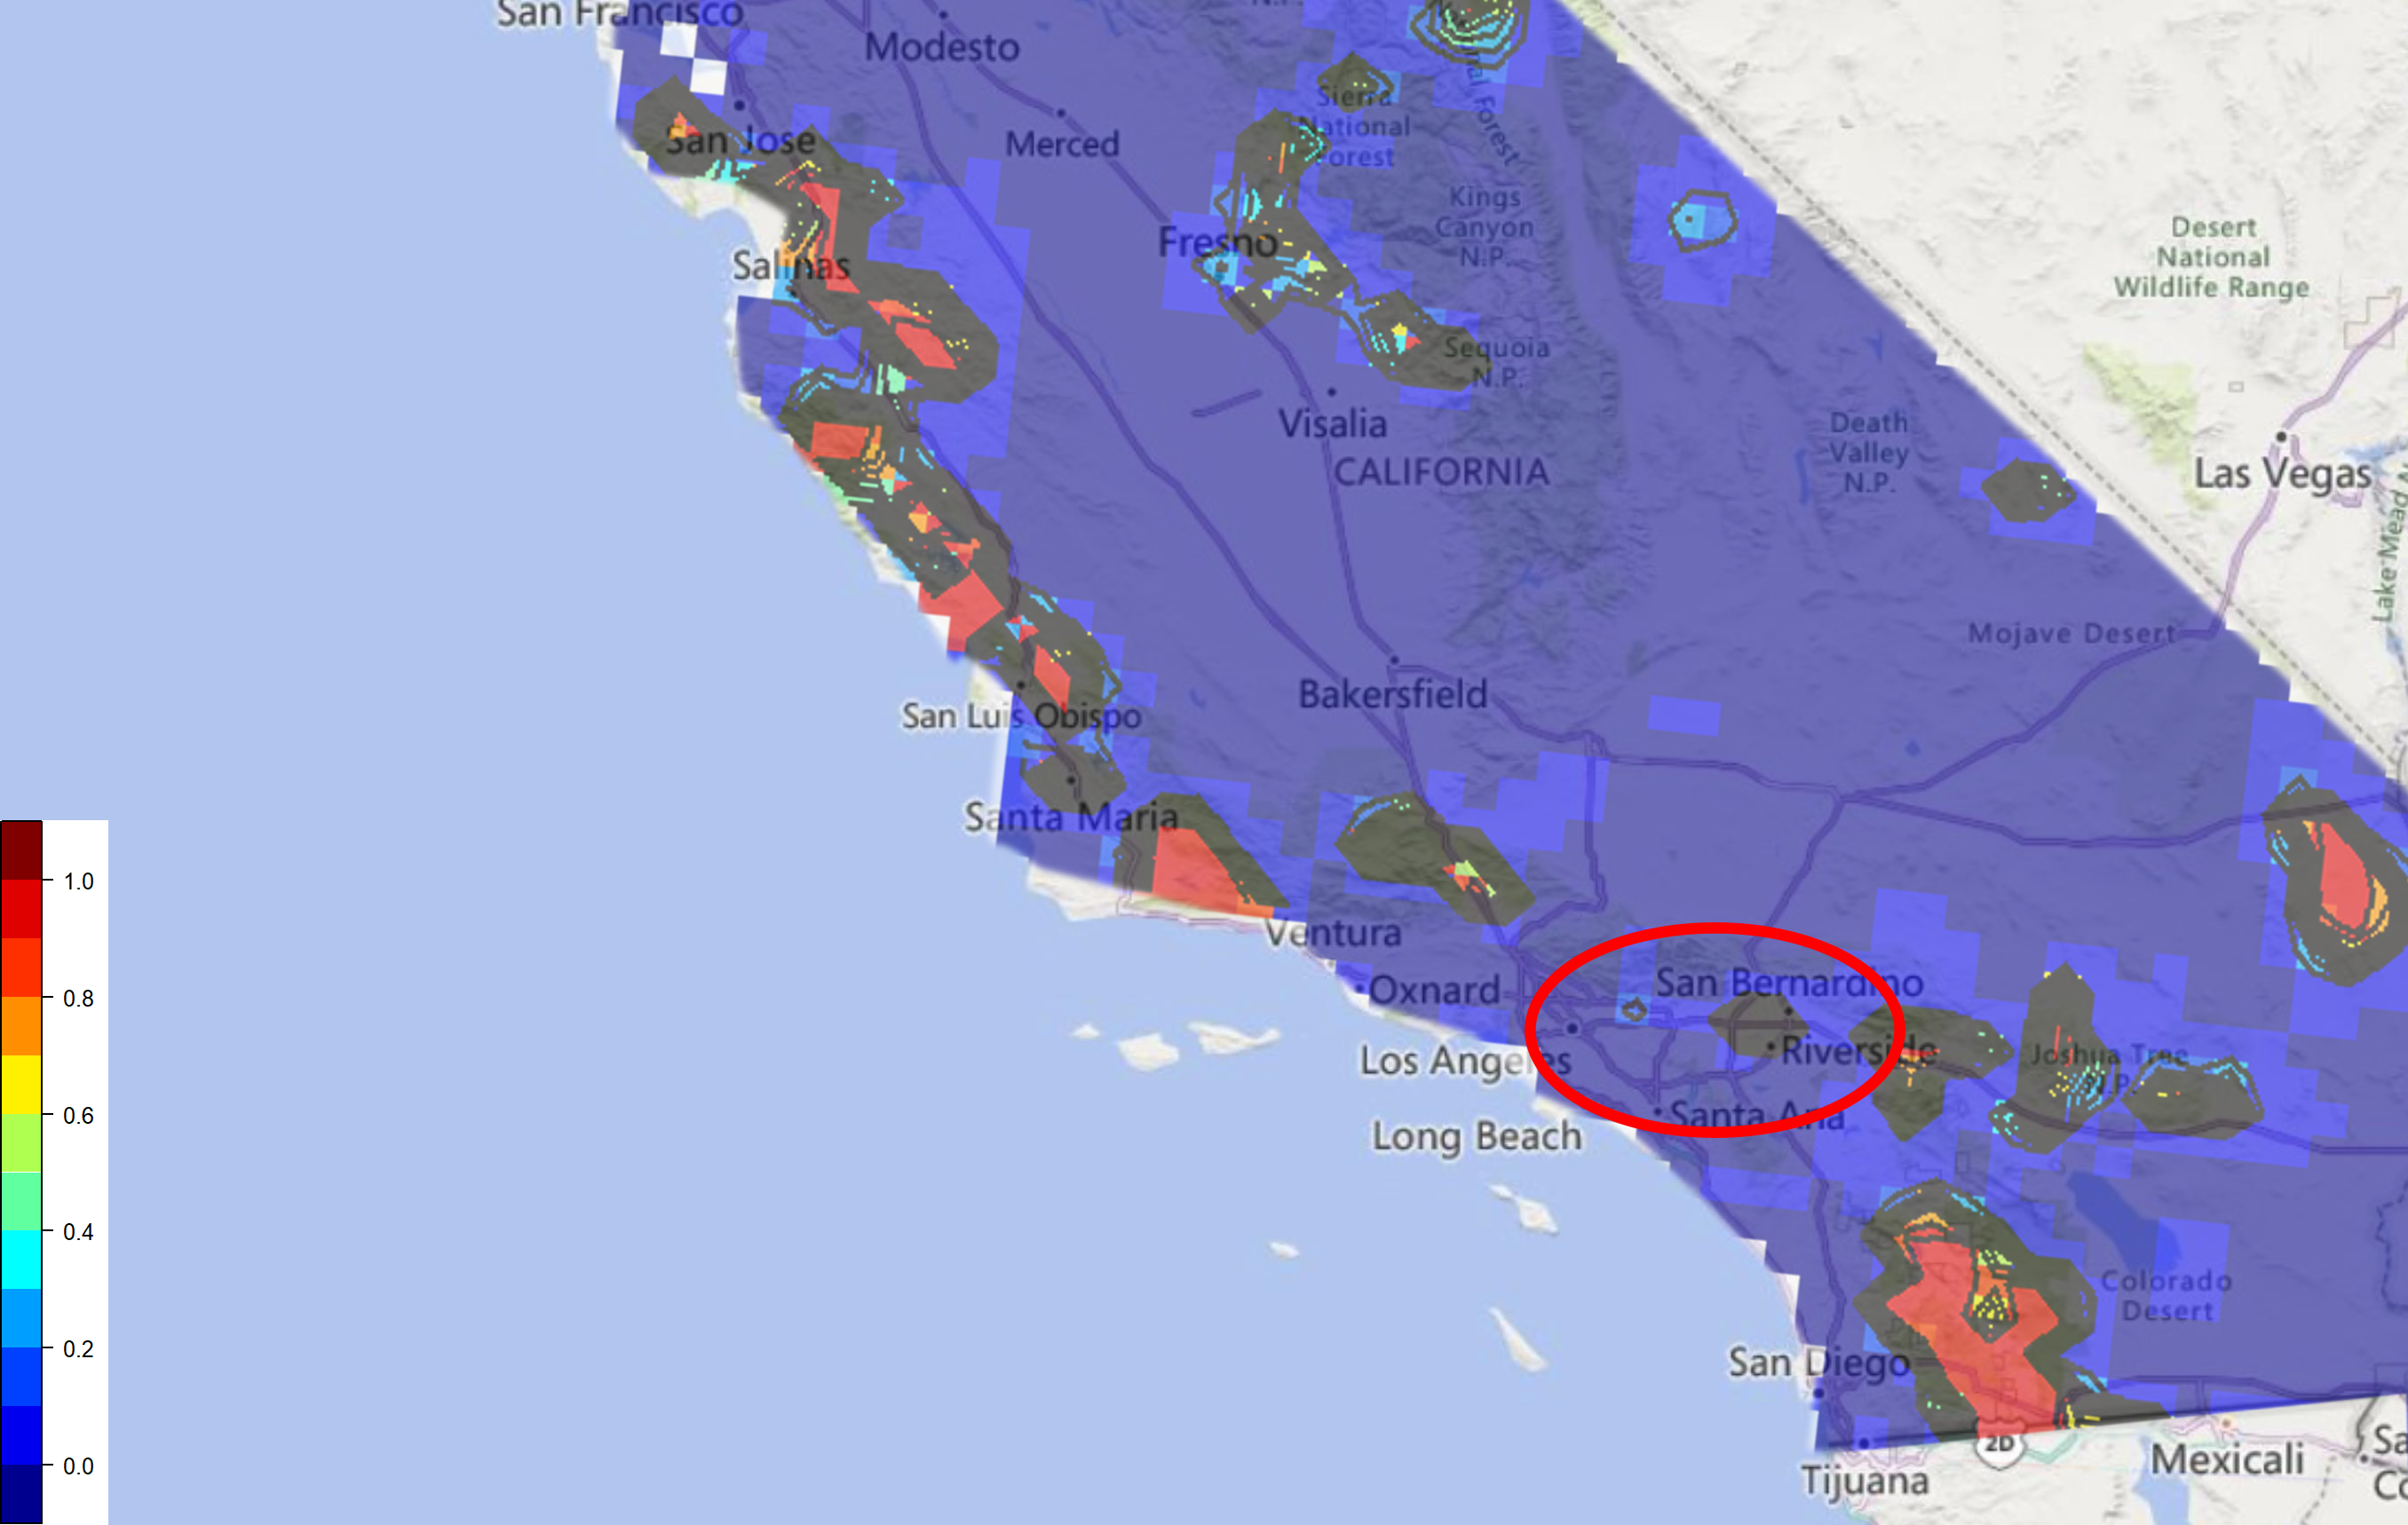
\includegraphics[width=0.5\textwidth]{images/qwq1.png}
    \caption{Excursion function for Urban community}
    \label{pre1}
\end{figure}

After comparing three reasonable decisions for the urban areas, from which we targeted the values of UES, PM2.5 and SO2 for the four urban regions including(LA,SB,R,S). We succeeded in obtaining a new model result, where coefficients including $\beta_{UES}$, $\beta_{PM2.5}$, and $\beta_{SO2}$, the posterior of the coefficient of UES shows the most significant change. In particular, the posterior distribution of the coefficient of UES is reduced to 37.5 $\%$ of the previous value, indicating that the\textbf{ policy for UES has the greatest impact on SQM} in this additive model. Here, we still use the excursion function to illustrate the probability that some areas in southern California jointly exceed the risk level of SQM, and we can find that the areas that exceed the level specified by light pollution are significantly smaller, which also indicates that our policy has completed its effective intervention.





\section{Model evaluation index}

\subsection{Model Cross validation}
In the process of developing statistical models, cross-validation is a crucial technique for evaluating the quality of the frameworks. In this case, we extract 110 locations with comparable geographic data, and each point has associated SQM observations. 10 random points' values are now changed to NA. The legend is provided below in order to accomplish our LGM model's goal of NA prediction and monitor our model's precision and strength  Results prove the model's fitting and prediction is effective and outstanding.

\begin{figure}[htp]
    \centering
    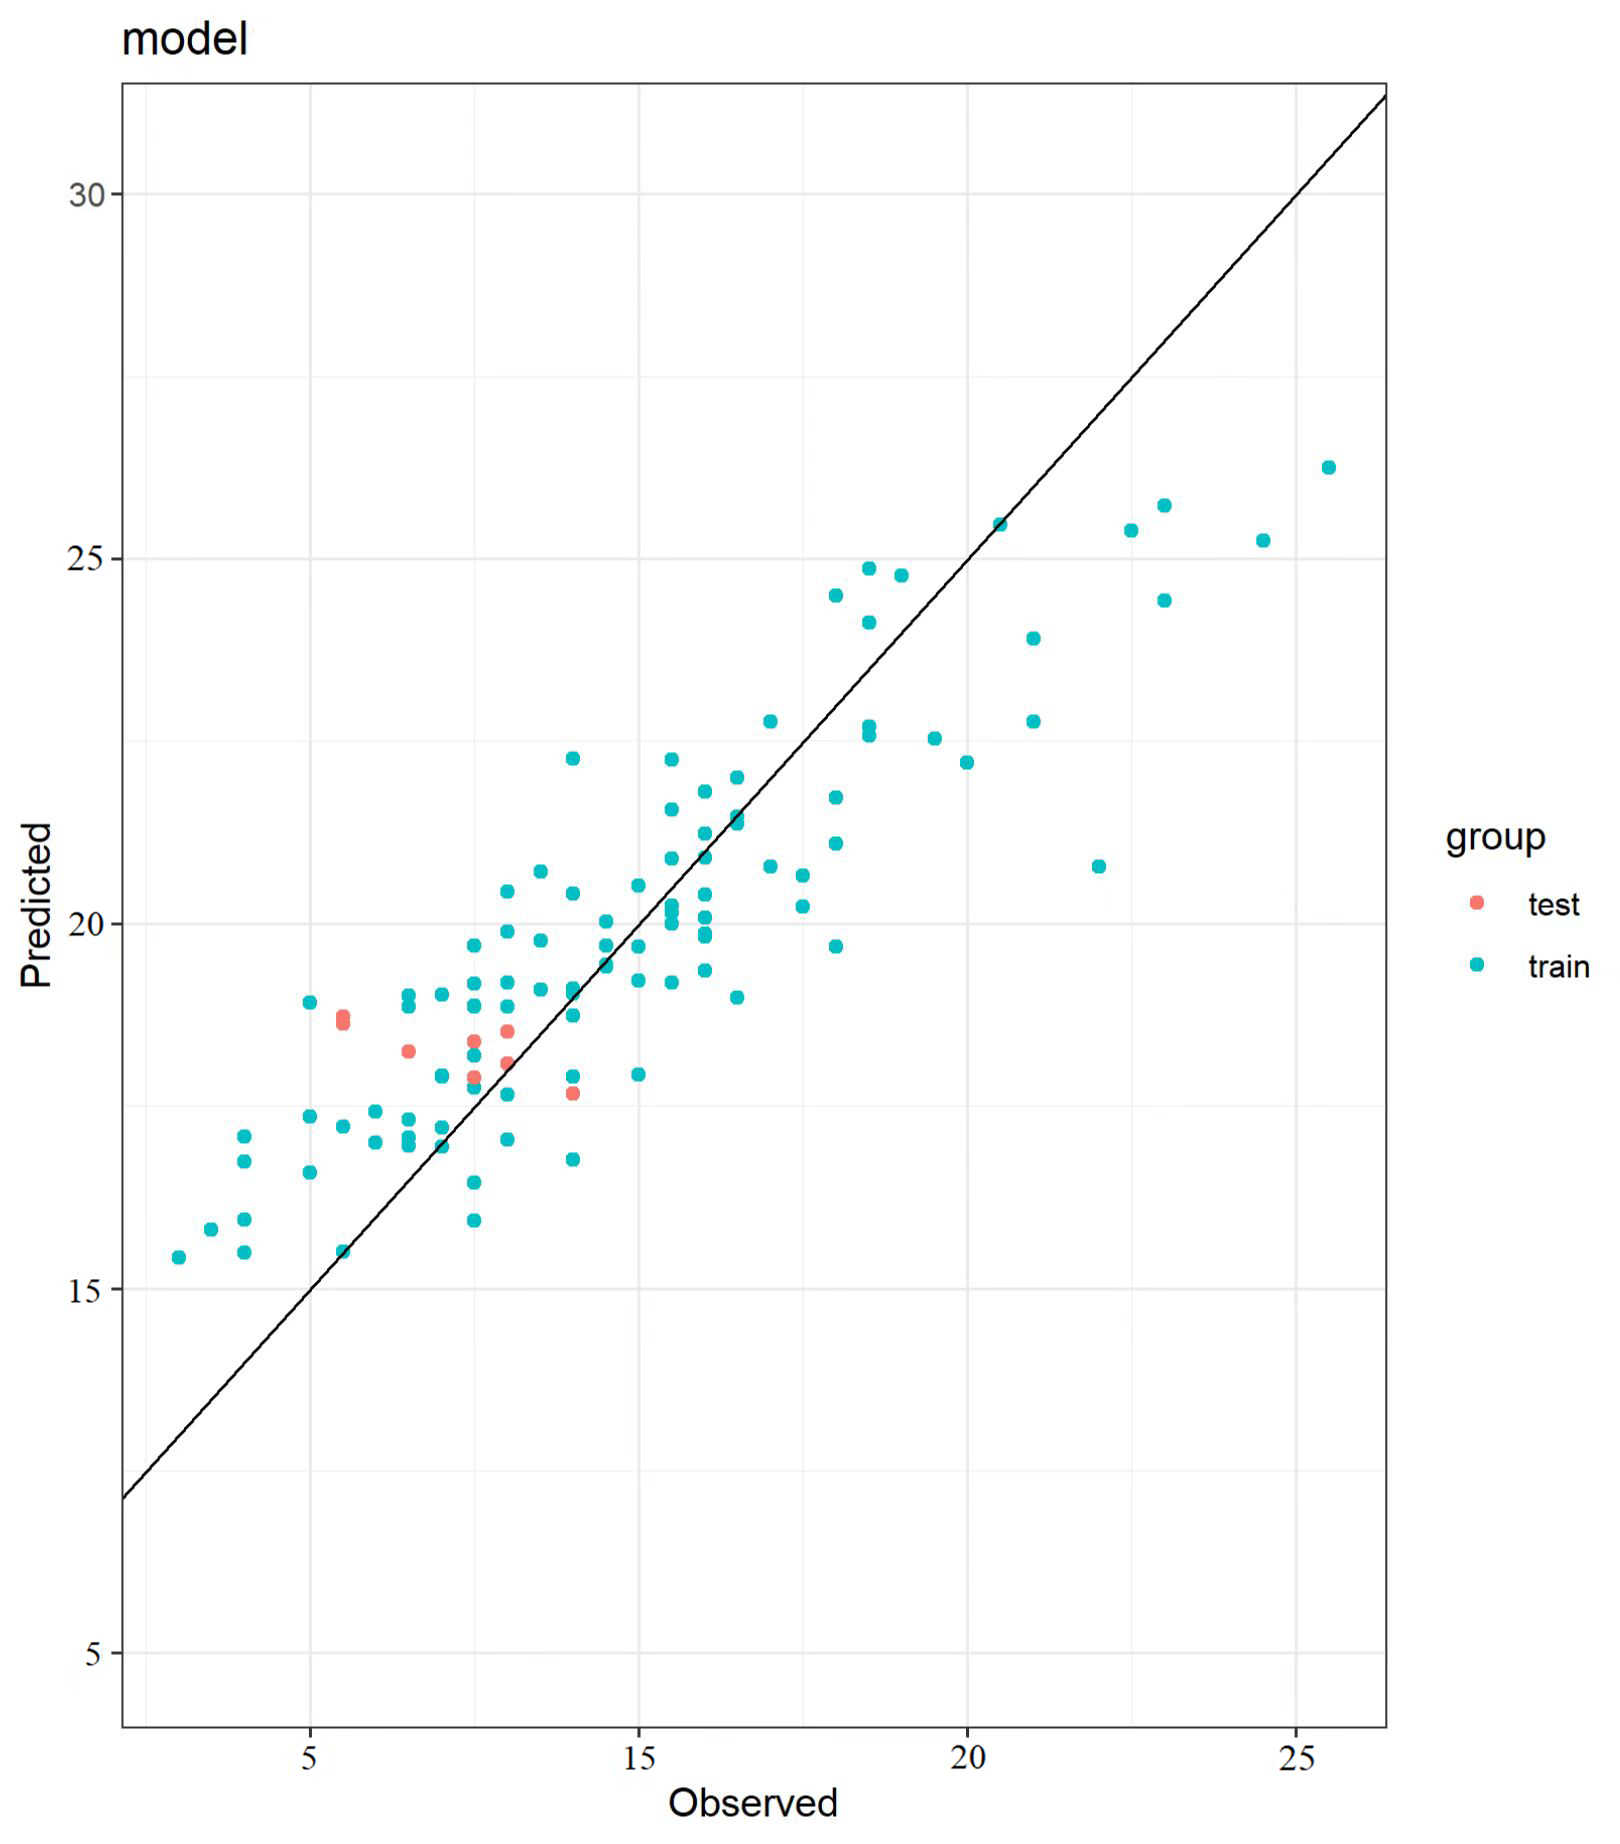
\includegraphics[width=0.5\textwidth]{images/training.png}
    \caption{Training and testing sets}
    \label{pre1}
\end{figure}

\subsection{Deviance Information Criterion (DIC)}
The deviance is typically used to compare models for generalized linear models (GLMs). Its formal definition is:

$$
D(\boldsymbol{\theta})=-2 \log (l(\boldsymbol{y} \mid \boldsymbol{\theta}))
$$

where  $l(\boldsymbol{y} \mid \boldsymbol{\theta}))$  is the likelihood and  $\boldsymbol{\theta}$  is the distribution you assign to your data. The smaller the deviance, the better the model in particular. The problem with the deviance is that the more complex the model (e.g. the more predictors it has), the smaller the deviance becomes (although after a certain point, the changes are minimal). This has led to the development of methods that penalize the deviance to account for model complexity (e.g. by accounting for the number of parameters in the model). The most common measure used in Bayesian contexts is the Deviance Information Criterion (DIC). The basis for the DIC is the posterior expected mean of the deviance  $E(D(\theta)$ . To this we add a penalty term, the effective number of parameters  $p_{D}$ . The idea of the  $p_{D}$  is that it is a measure of the number of parameters that are being used by the model.

\subsection{Widely Applicable Information Criterion (WAIC)}
WAIC is a more fully Bayesian approach for estimating the out-of-sample expectation based on the log pointwise posterior predictive density. WAIC is an estimate of out-of-sample relative K-L divergence (KLD), and it is defined as:

$$
WAIC=-2(lppd-pWAIC)
$$

Components  $lppd$  (log pointwise predictive density) and  $pWAIC$  (the effective number of parameters) are reported as attributes.

DIC is 12130.44 and WAIC 12285.26.

\subsection{The probability integral transform (PIT).}

\begin{figure}[htp]
    \centering
    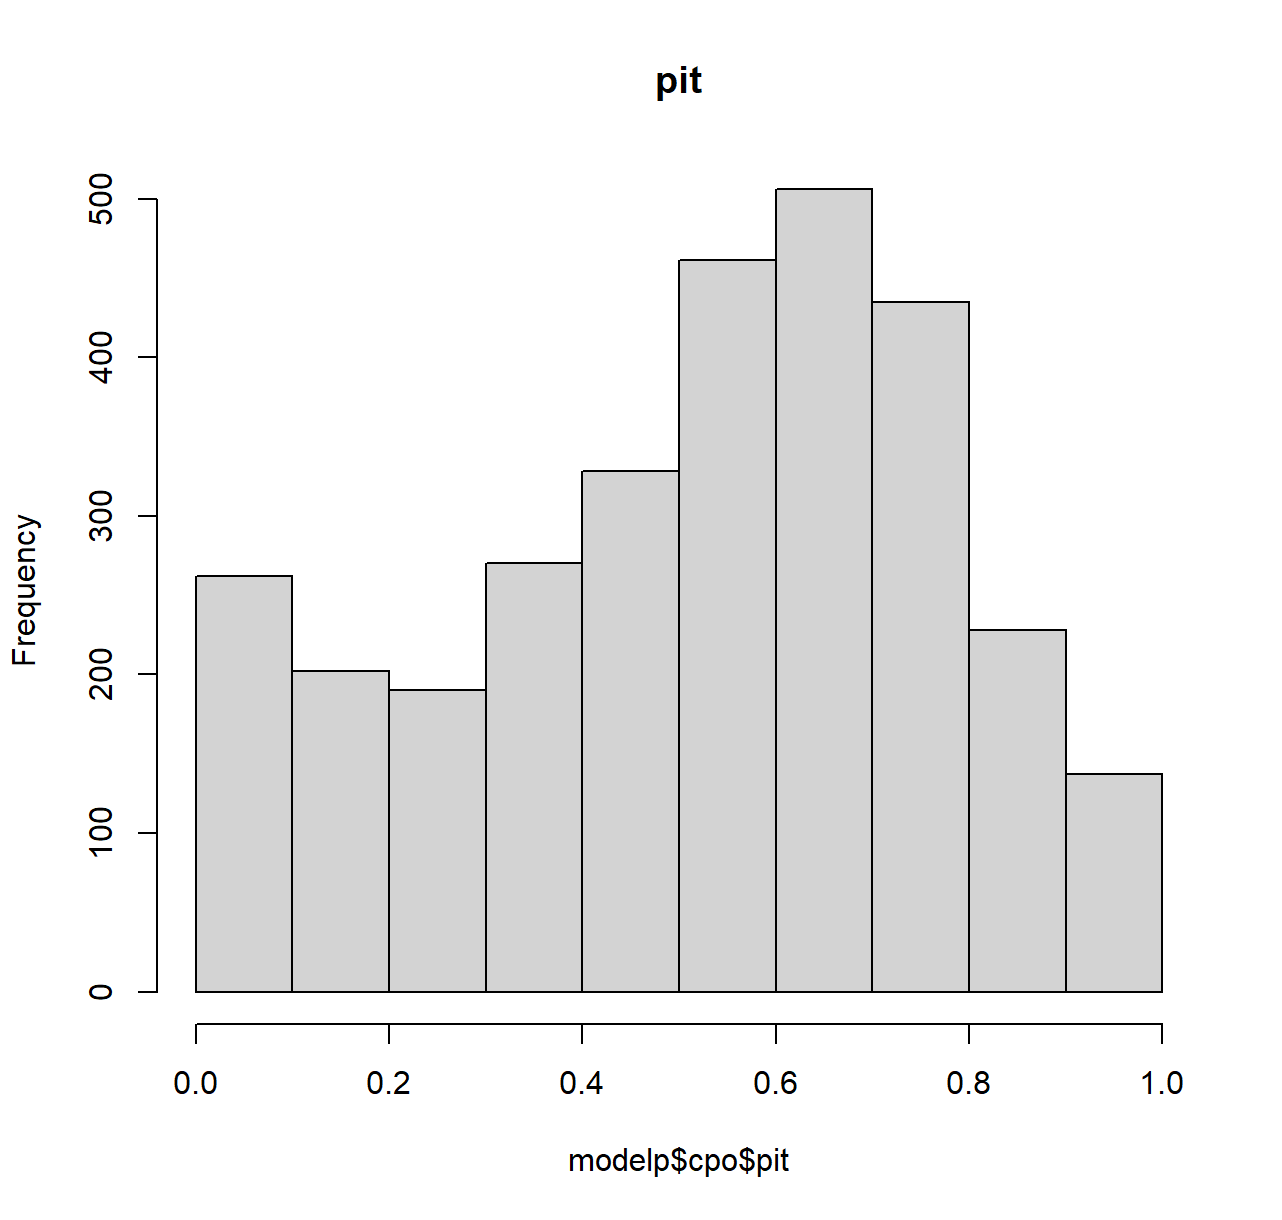
\includegraphics[width=0.5\textwidth]{images/ppt11111.png}
    \caption{Excursion function for Rural community}
    \label{pre1}
\end{figure}

$$
PIT=p\left(y_{i}^{p}<y_{i} \mid \boldsymbol{y}_{-i}\right)
$$

For different  $y_{i}^{p}$  and if this is approximately uniform, then the model fits the data well, otherwise, it is probably misspecified.

\subsection{Strengths and limitations}

\subsubsection{Strengths}

\begin{itemize}
	
\item Based on the geographical distribution of observation points in California, our model implements the spatial modeling based on GMRF and SPDE approach, and specifically explains the spatial correlation of observation quantity SQM under the influence of covariables. Compared with the iid case of traditional regression model, the spatial correlation is better used to explain the random effects between each other.  

\item LGM is used under the framework of Bayesian inference and INLA method, so as to process the predicted value of the model more quickly and efficiently.

\item In the process of the three decisions, the additive model processes the covariable data to have a certain amount of impact on the decision results.

\item Using the excursion function and excursion set, the range of an area that exceeds a risk level and the probability that this area exceeds the risk level are determined. Then explain the formation of the actual governance of SQM.

\end{itemize}

\subsubsection{limitations}
\begin{itemize}
\item Data limitation: During the process of data collection and intrinsic hindrance for large and comprehensive whole scale data set, we are only able to collected a limited amount of data points in the Southern California.
\item Computational Power limitation: Spatial modeling using R-INLA package requires high computational power and GPU resources for larger data set and more accurate measurement of impacts of intervention strategy for light pollution.

\end{itemize}

\newpage
\begin{thebibliography}{99}
\bibitem{1} Oak Ridge National Laboratory, LandScan™, http://web.ornl.gov/sci/landscan/ [accessed May 28, 2016].

\bibitem{2} Light Pollution Map, Lightpollutionmap.info, https://www.lightpollutionmap.info/

\bibitem{3} Falchi, Fabio; Cinzano, Pierantonio; Duriscoe, Dan; Kyba, Christopher C. M.; Elvidge, Christopher D.; Baugh, Kimberly; Portnov, Boris; Rybnikova, Nataliya A.; Furgoni, Riccardo (2016). Supplement to: The New World Atlas of Artificial Night Sky Brightness. GFZ Data Services. http://doi.org/10.5880/GFZ.1.4.2016.001

\bibitem{4} Falchi F, Cinzano P, Duriscoe D, Kyba CC, Elvidge CD, Baugh K, Portnov BA, Rybnikova NA, Furgoni R. The new world atlas of artificial night sky brightness. Science Advances. 2016 Jun 1;2(6):e1600377.

\bibitem{5} Light pollution datasets in 2020, https://www.globeatnight.org/maps.php

\bibitem{6} California GDP datasets in 2020, https://california.reaproject.org/data-tables/gsp-a200n/csv/

\bibitem{7} California PM2.5 datasets in 2020, https://www.epa.gov/outdoor-air-quality-data/download-daily-data

\bibitem{8} 2020 California SO2 pollutant report, https://www.epa.gov/outdoor-air-quality-data/monitor-values-report-hazardous-air-pollutants

\bibitem{9}  NASA's VIIRS/NPP Lunar BRDF-Adjusted Nighttime Lights Yearly, https://ladsweb.modaps.eosdis.nasa.gov/missions-and-measurements/products/VNP46A4

\bibitem{10} Wojciech Banaszczyk. On a certain class of positive definite functions and measures on locally compact Abelian groups and inner-product spaces. Journal of Functional Analysis. \\https://doi.org/10.1016/j.jfa.2021.109261.

\bibitem{10} Philip Lawrence and Antonia McBride and Laurie McCartney and Rebecca Thursfield. Measuring Respiratory Function, Encyclopedia of Respiratory Medicine (Second Edition). 2022 ISBN:978-0-08-102724-0. \\https://doi.org/10.1016/B978-0-08-102723-3.00243-2.

\bibitem{11} Uwes Anis Chaeruman, Basuki Wibawa, and Zulfiati Syahrial. Determining the Appropriate Blend of Blended Learning: A Formative Research in the Context of Spada-Indonesia. http://dx.doi.org/10.12691/education-6-3-5.

\bibitem{12} Yasuyuki Hamura and Tatsuya Kubokawa. Bayesian predictive density estimation for a Chi-squared model using information from a normal observation with unknown mean and variance. \\https://doi.org/10.1016/j.jspi.2021.07.004.

\bibitem{13} Nuran Peker and Cemalettin Kubat. Application of Chi-square discretization algorithms to ensemble classification methods. \\https://doi.org/10.1016/j.eswa.2021.115540.

\end{thebibliography}

\begin{figure}
    \centering
    
\includegraphics[width=0.9\textwidth]{57f45a1dbd44a(suo).png}
    \caption{Flyer to promote intervention strategy in light pollution with special attention to Urban Electricity Supply--for urban location in LA, California}
    \label{fig:my_label}
\end{figure}

\end{document}
%% 
%% This work consists of these files mcmthesis.dtx,
%%                                   figures/ and
%%                                   code/,
%% and the derived files             mcmthesis.cls,
%%                                   mcmthesis-demo.tex,
%%                                   README,
%%                                   LICENSE,
%%                                   mcmthesis.pdf and
%%                                   mcmthesis-demo.pdf.
%%
%% End of file `mcmthesis-demo.tex'.
